% -*- coding: utf-8 -*-

\documentclass[a4paper,dvipdfmx]{jsarticle}
\usepackage{ascmac,alltt,txfonts,url}

\usepackage[dvipdfmx]{graphicx}
\usepackage{here}
\usepackage{fancyvrb}

\renewcommand{\ttdefault}{cmtt}
\renewcommand{\figurename}{図} 
\renewcommand{\tablename}{表} 
\DeclareMathAlphabet{\mathtt}{OT1}{cmtt}{m}{n}
\SetMathAlphabet{\mathtt}{bold}{OT1}{cmtt}{m}{n}
\setlength{\oddsidemargin}{0cm}
\setlength{\evensidemargin}{0cm}

\makeatletter

\newdimen\@mojihaba
\settowidth{\@mojihaba}{あ}

\def\tokushu#1{%
\def\tokushutitle{#1}%
\gdef\articleHeader{\hbox to\textwidth{\rule{3\@mojihaba}{1mm}%
\hbox{\small\bf\hskip1mm \tokushutitle}\leaderfill}}
}

\newdimen \JQ	\JQ .259817mm	%%%	\JQ/\Q = 10pt/9.62216pt
\newdimen \Q	\Q  .25mm	%%%	Quarter of 1mm

\def\JarticleHeader{\rule{\textwidth}{1mm}}%
\def\JarticleTitle{{\huge\bf\@title}}
\def\JarticleAuthor{\large\begin{tabular}[t]{@{}l}\@author\end{tabular}}
\newbox\@temptitlebox

\def\verse{\let\\=\@centercr 
 \list{}{\itemsep\z@ \itemindent -1.5em\listparindent \itemindent 
 \rightmargin\leftmargin\advance\leftmargin 1.5em}\item[]}
\let\endverse\endlist
\def\quotation{\list{}{\listparindent 1.5em
 \itemindent\listparindent
 \rightmargin\leftmargin \parsep 0pt plus 1pt}\item[]}
\let\endquotation=\endlist
\def\quote{\list{}{\rightmargin\leftmargin}\item[]}
\let\endquote=\endlist
\def\abstquotation{\list{}{\listparindent 1.5em
 \itemindent\listparindent
 \leftmargin 5mm
 \rightmargin\leftmargin \parsep 0pt plus 1pt}\item[]}
\let\endabstquotation=\endlist
\def\quote{\list{}{\rightmargin\leftmargin}\item[]}
\let\endquote=\endlist

\global\def\@maketitle{\newpage \null
\hbox{\vbox to193.5\Q{\baselineskip=10mm % 193.5\Q = 9*\baselineskip
\begin{flushleft}
\JarticleHeader
% following extra vskip together with baselineskip(10mm) will produce
% appropriate 10mm/6mm gap between the rule and title
% This assumes that title is typeset with 28Q(7mm) font, and baseline
% is set 1mm above the bottom of the font.
\setbox\@temptitlebox\hbox{JarticleTitle}\ifdim\wd\@temptitlebox>\textwidth\vskip2mm\else\vskip6mm\fi
\leftskip=5mm
\JarticleTitle
\vskip6mm % to leave 10mm gap between title and author
\JarticleAuthor
\end{flushleft}\vfil}}
%\JEabstInsert
  \begin{small}
    \begin{abstquotation}
      \Jabstcontent
    \end{abstquotation}
  \end{small}
}

\long\def\Jabstract#1{\global\long\def\Jabstcontent{\noindent\ignorespaces #1}}
\def\Jabstcontent{\relax}

\makeatother

\usepackage{fancyhdr}
\pagestyle{fancy}
\lhead{Vivadoを使ったFPGA開発 クイックスタート}
\rhead{}
\rhead{\thepage{}}
\cfoot{}
\renewcommand{\headrulewidth}{0.5pt}
\pagestyle{fancy}

\Jabstract{%
\\
FPGA開発におけるHello World ``Lチカ'' を通して,開発の手順に慣れよう
}

\begin{document}

\title{Vivadoを使ったFPGA開発 クイックスタート}
\author{}
\date{2019年 1月14日~~第3.0版}
\maketitle

\section{はじめに}
この章では,FPGA開発におけるHello World,すなわち最初に試してみるサンプルとして``Lチカ''を題材に,開発の手順に慣れてみましょう.``Lチカ''とは,「LEDをチカチカさせる」の略です.

単にLEDとチカチカさせるだけ,なのですが,開発の手順を身につけるには十分です.また,実際多くの信号制御は何かしらの規則にしたがって信号をON/OFFしていることですから,すべての信号制御はLチカの応用にあるとも言えます.簡単ですが大事ですよ.

\section{実習}

\subsection{プロジェクトの用意}


 \begin{figure}[H]
  \begin{center}
   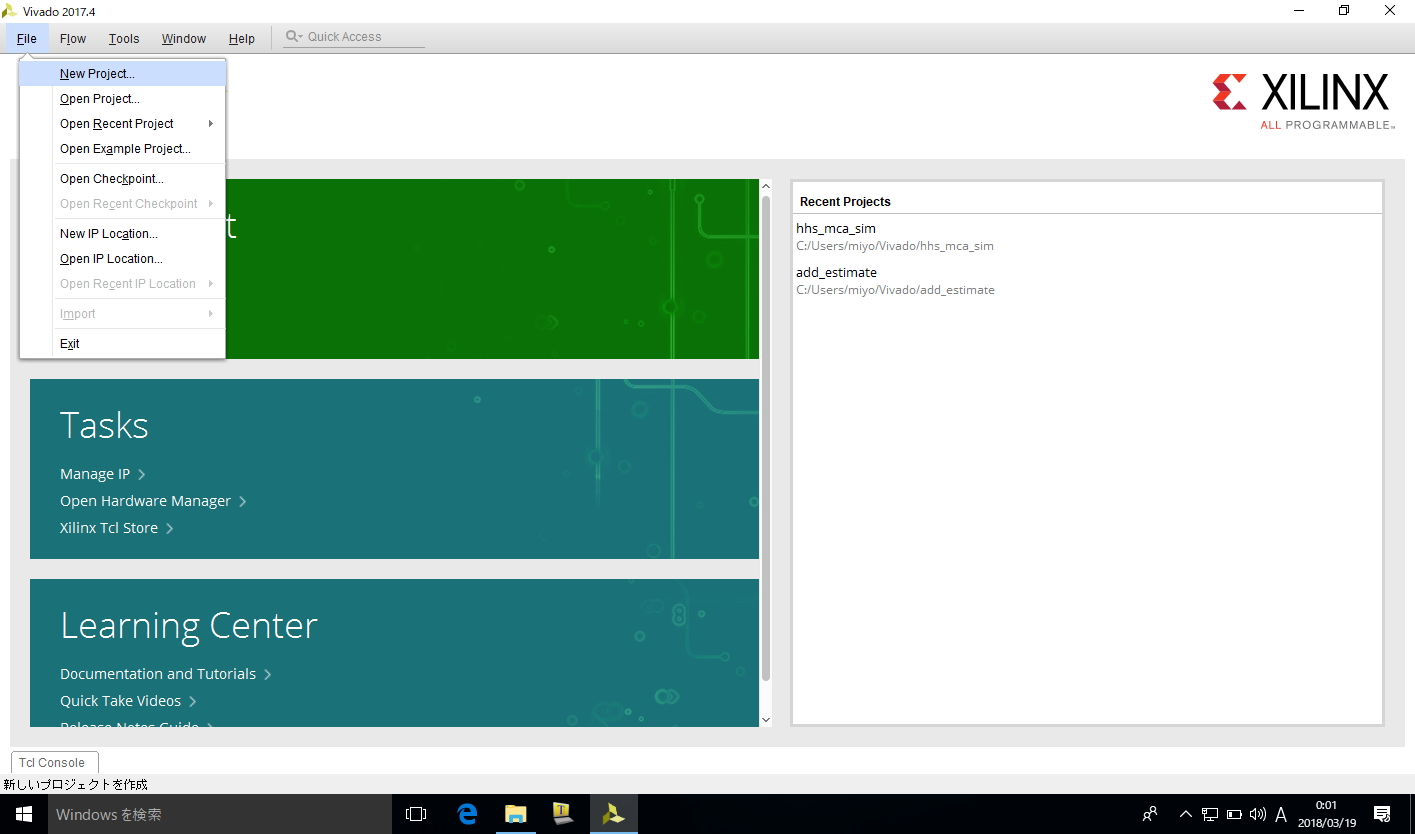
\includegraphics[width=.8\textwidth]{chapter03_figures/VirtualBox_Windows10_19_03_2018_00_01_24.png}
  \end{center}
  \caption{VivadoのFileメニューから,New Project...を選択する}
 \end{figure}

 \begin{figure}[H]
  \begin{center}
   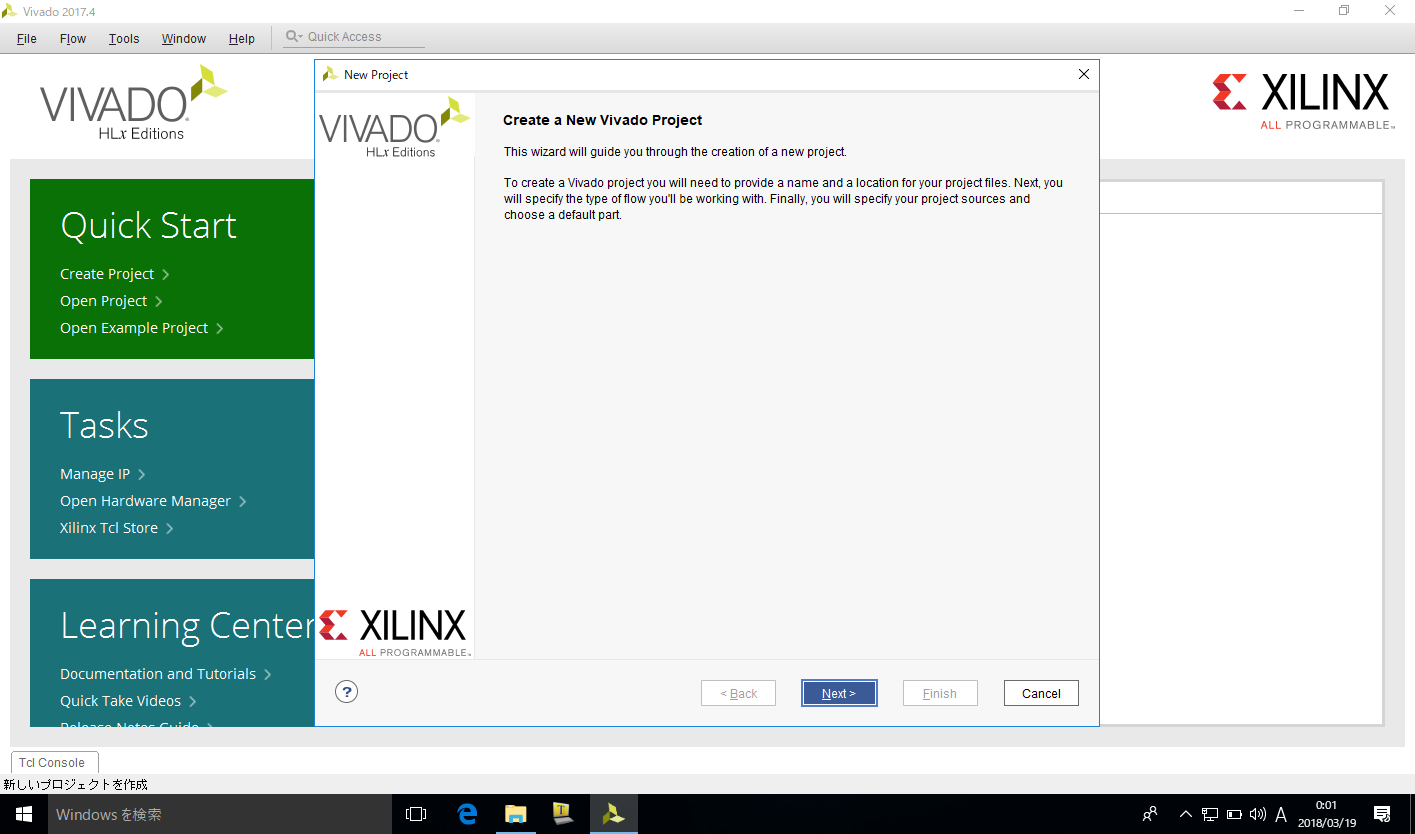
\includegraphics[width=.8\textwidth]{chapter03_figures/VirtualBox_Windows10_19_03_2018_00_01_32.png}
  \end{center}
  \caption{プロジェクト作成ダイアログが開くので,Next$\gt$で次へ}
 \end{figure}

プロジェクト名と格納先を決めます.ここでは,ホームディレクトリの下のVivadoというフォルダの下にプロジェクトを格納することとし,名前をproject\_1としています.
 \begin{figure}[H]
  \begin{center}
   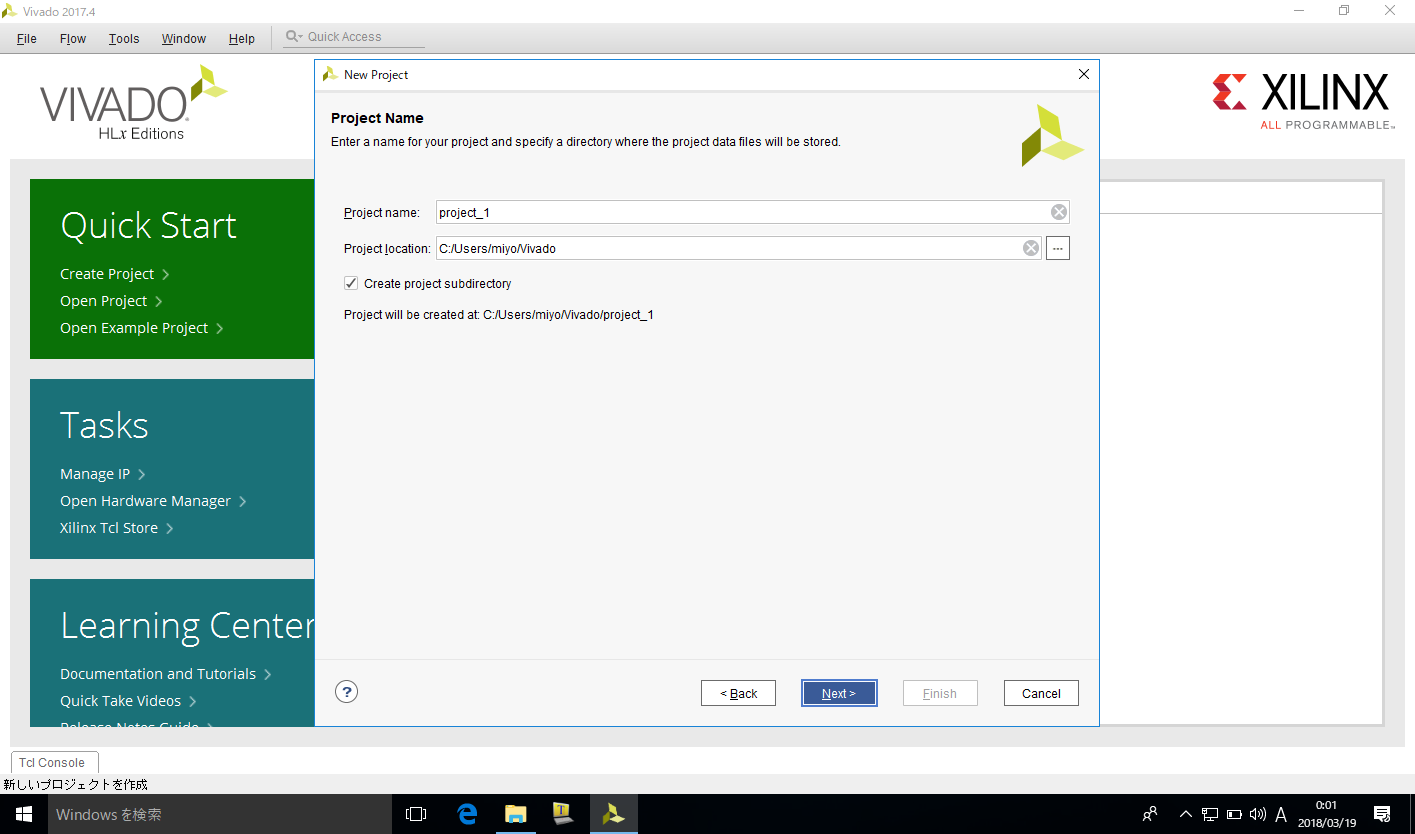
\includegraphics[width=.8\textwidth]{chapter03_figures/VirtualBox_Windows10_19_03_2018_00_01_37.png}
  \end{center}
  \caption{プロジェクト名と格納先を決めます}
 \end{figure}

 \begin{figure}[H]
  \begin{center}
   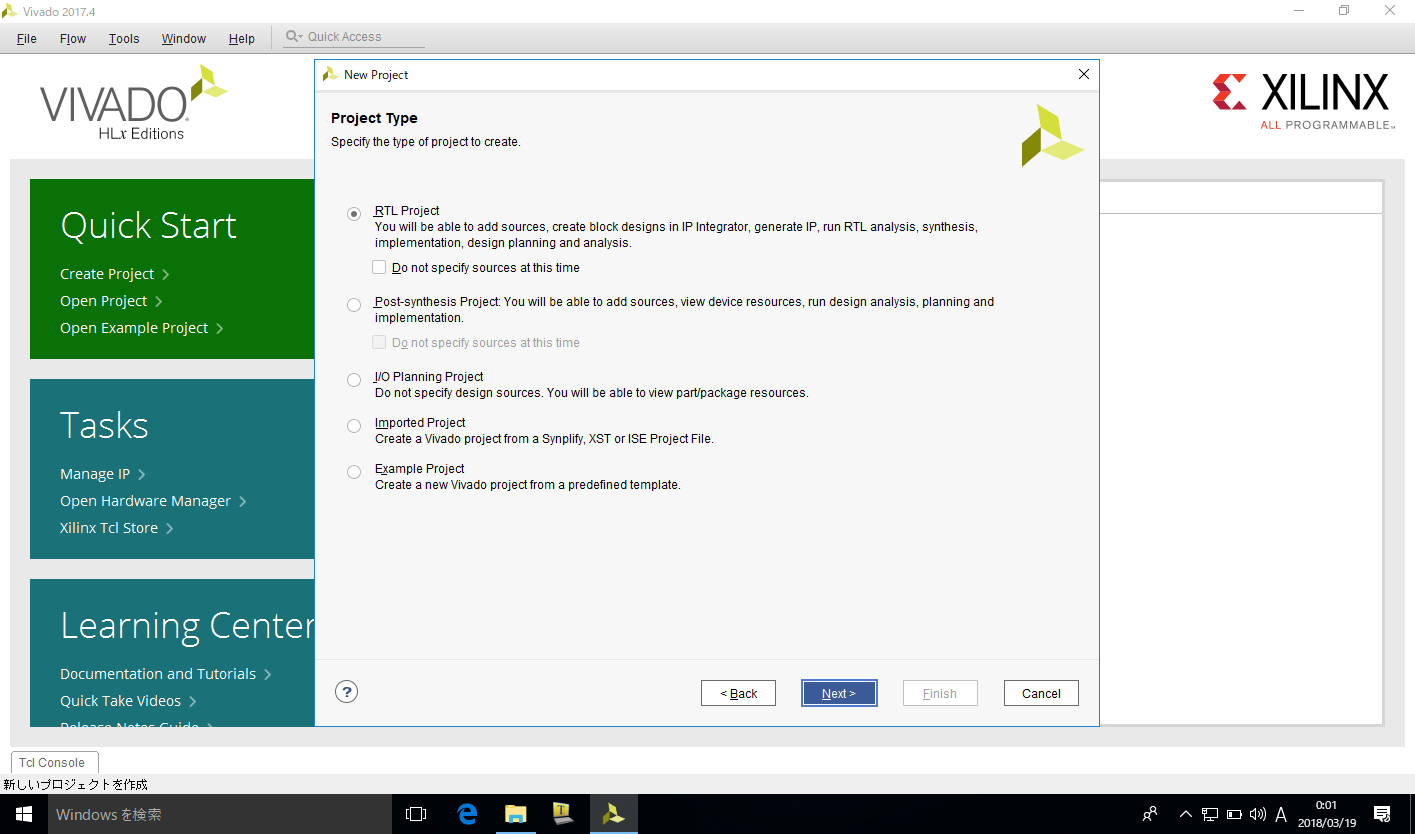
\includegraphics[width=.8\textwidth]{chapter03_figures/VirtualBox_Windows10_19_03_2018_00_01_43.png}
  \end{center}
  \caption{プロジェクトタイプの指定です.RTLプロジェクトを指定します}
 \end{figure}

 \begin{figure}[H]
  \begin{center}
   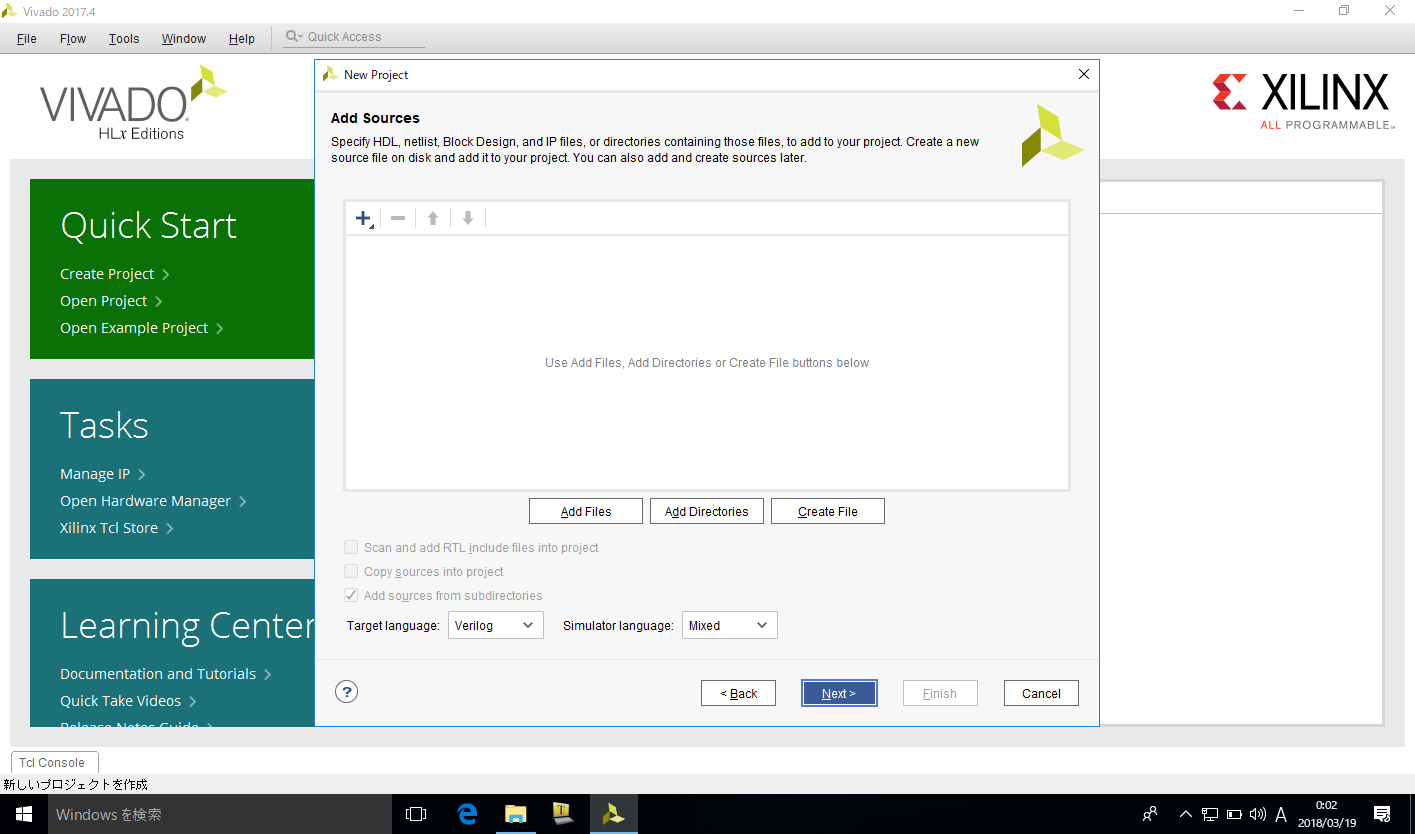
\includegraphics[width=.8\textwidth]{chapter03_figures/VirtualBox_Windows10_19_03_2018_00_02_24.png}
  \end{center}
  \caption{すでにソースコードがある場合にはここで追加できます.今回はないのでNext$\gt$で,そのまま次へ}
 \end{figure}

 \begin{figure}[H]
  \begin{center}
   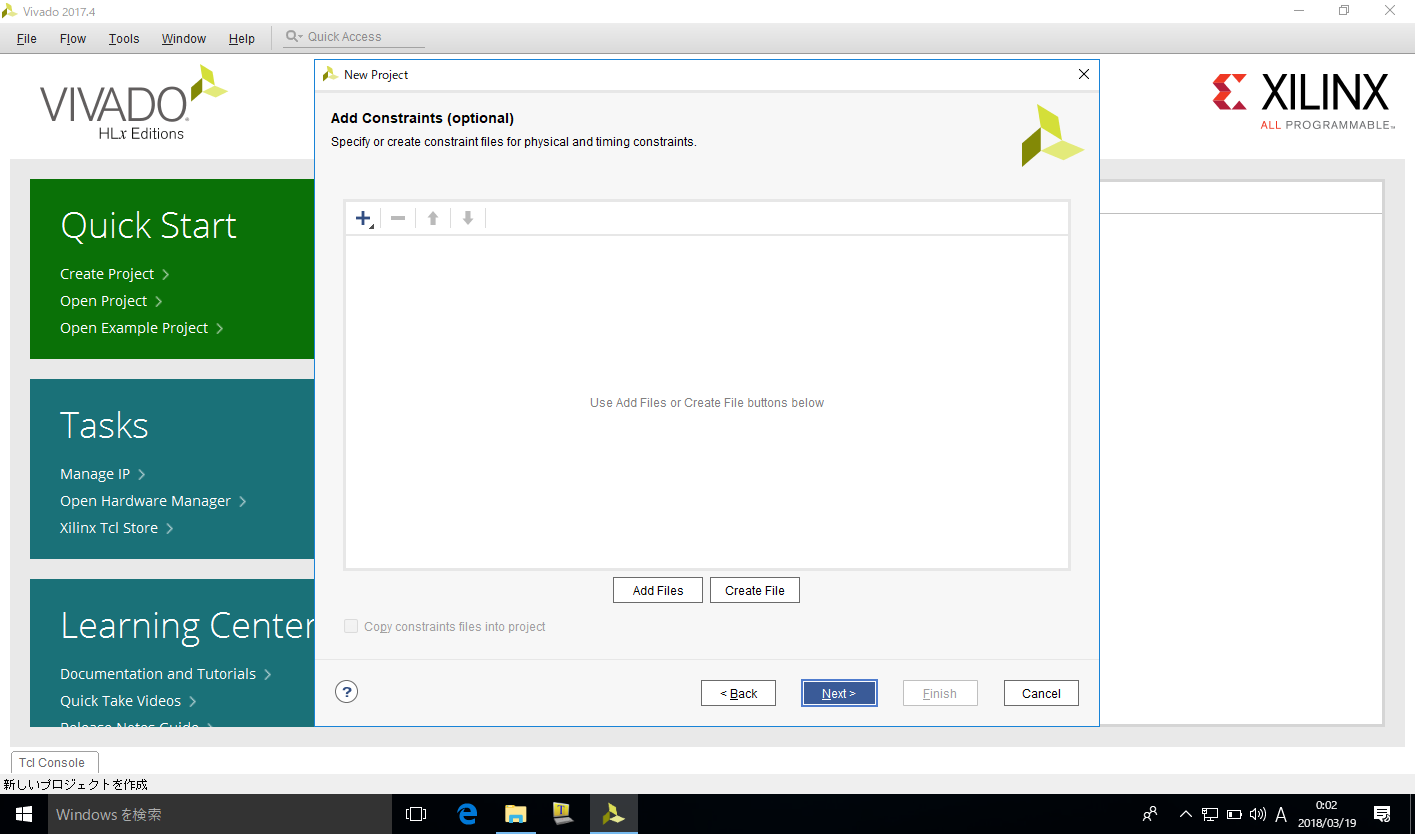
\includegraphics[width=.8\textwidth]{chapter03_figures/VirtualBox_Windows10_19_03_2018_00_02_30.png}
  \end{center}
  \caption{すでに制約ファイルがある場合にはここで追加できます.今回はないのでNext$\gt$で,そのまま次へ}
 \end{figure}

 \begin{figure}[H]
  \begin{center}
   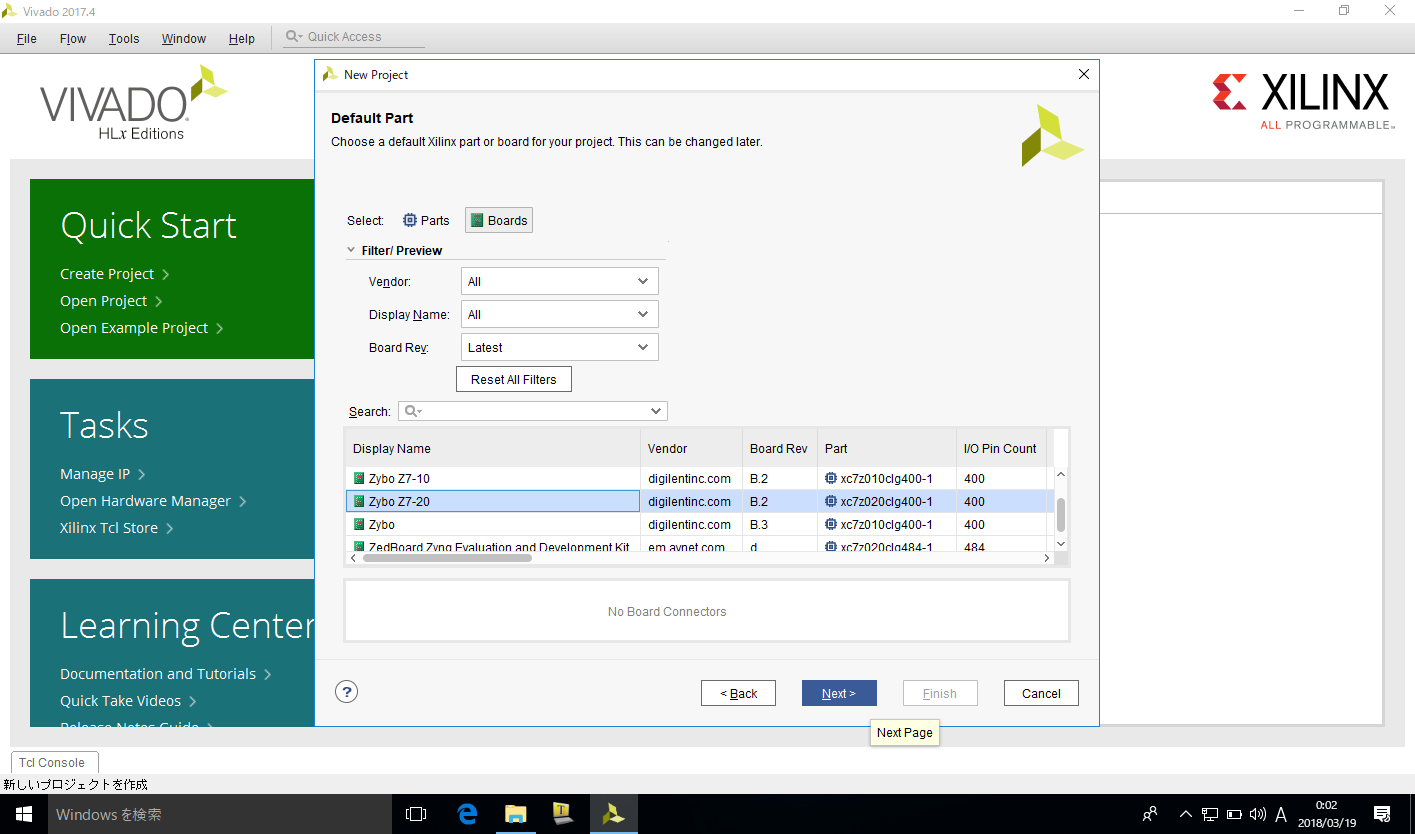
\includegraphics[width=.8\textwidth]{chapter03_figures/VirtualBox_Windows10_19_03_2018_00_02_49.png}
  \end{center}
  \caption{ターゲットとするFPGAの選択画面です.BoardタブをクリックしZybo Z7-20を選択して$\gt$で次へ}
 \end{figure}

 \begin{figure}[H]
  \begin{center}
   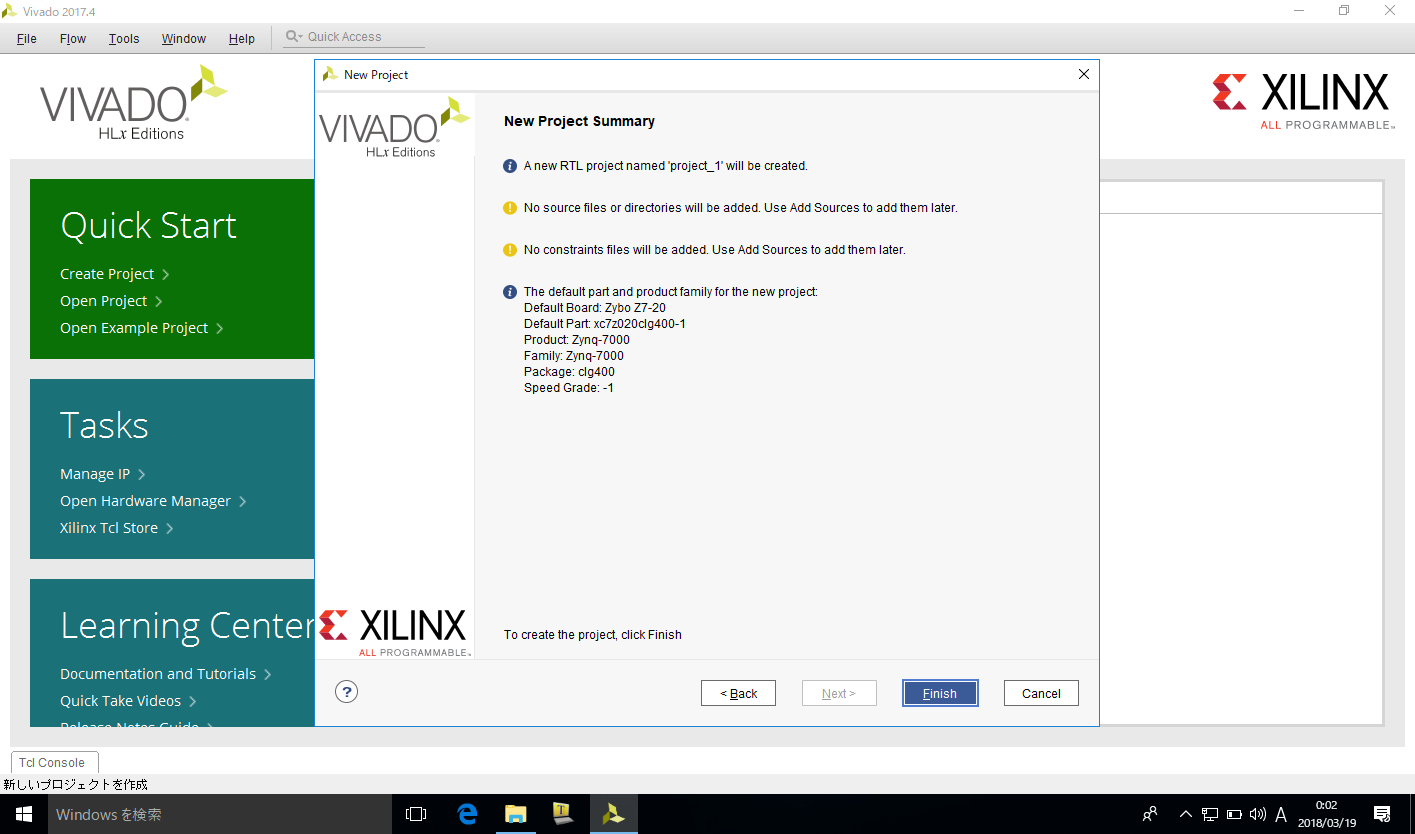
\includegraphics[width=.8\textwidth]{chapter03_figures/VirtualBox_Windows10_19_03_2018_00_02_55.png}
  \end{center}
  \caption{確認画面です.Finishをクリックするとプロジェクトの作成は完了です}
 \end{figure}

 \begin{figure}[H]
  \begin{center}
   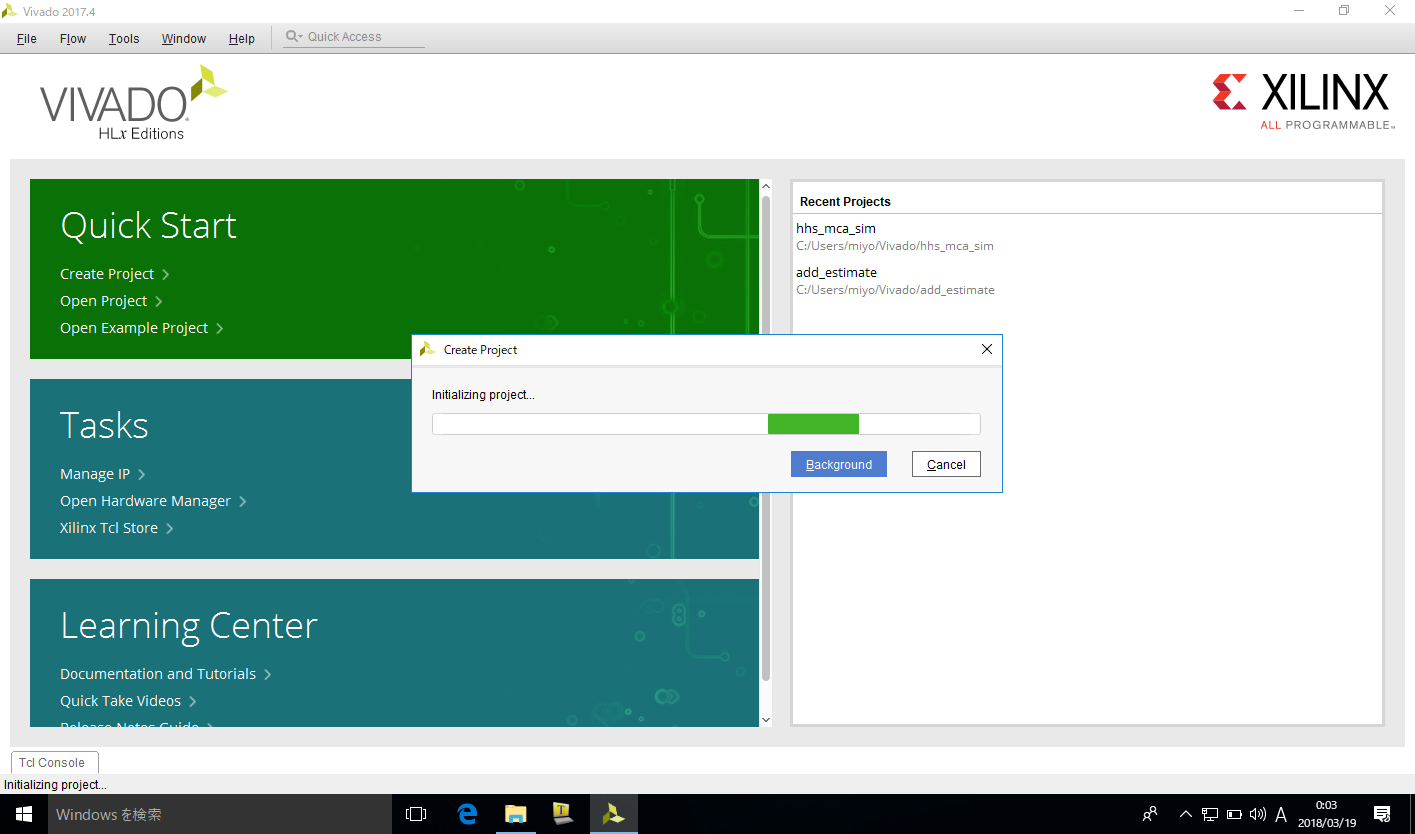
\includegraphics[width=.8\textwidth]{chapter03_figures/VirtualBox_Windows10_19_03_2018_00_03_06.png}
  \end{center}
  \caption{プロジェクト作成には少し時間がかかります}
 \end{figure}

これでプロジェクトの完成です.Product FamilyがZynq-7000に,Project Summaryの表示を見ると,Project partがZybo Z7-20と,Z7-20向けのプロジェクトができていることがわかります.
 \begin{figure}[H]
  \begin{center}
   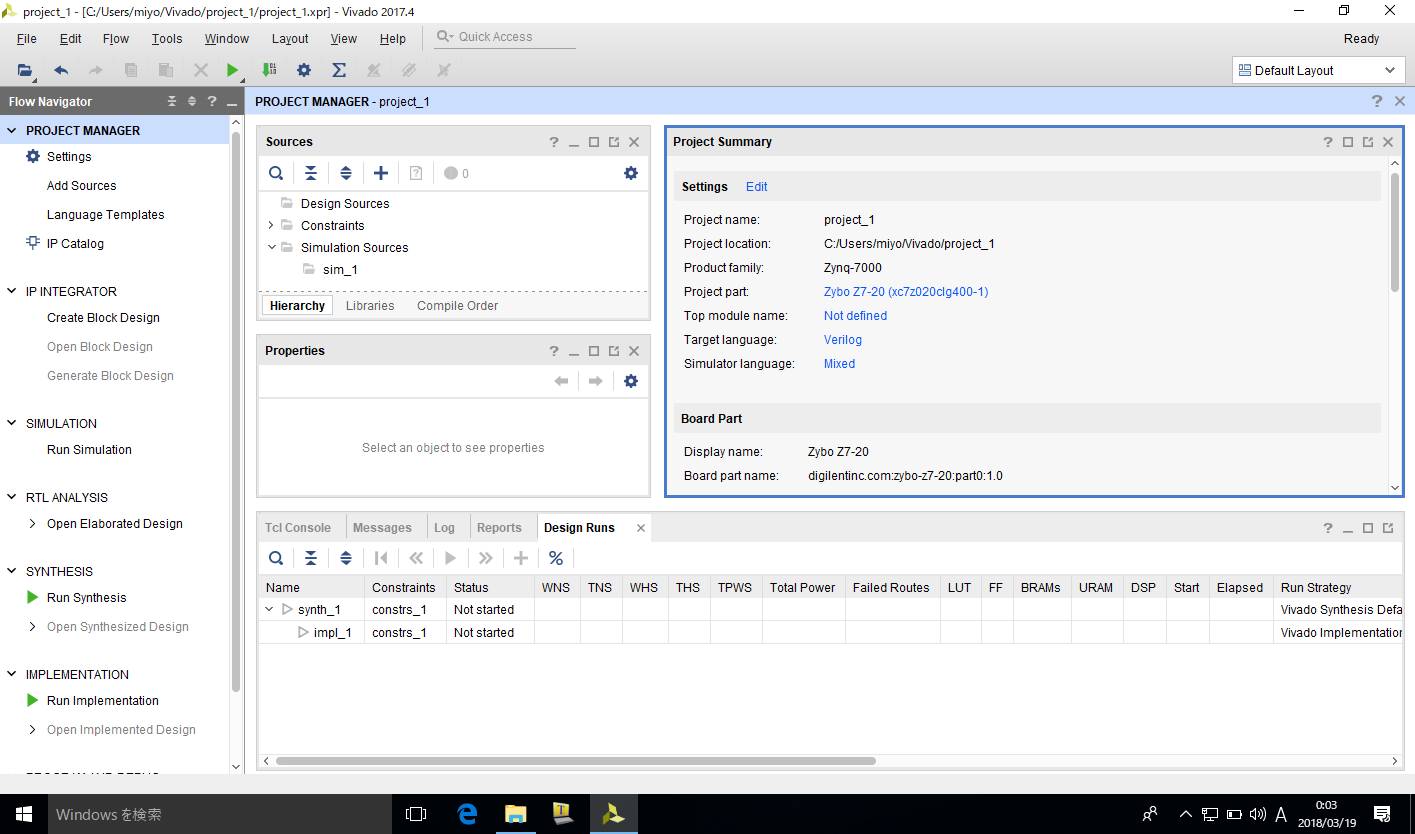
\includegraphics[width=.8\textwidth]{chapter03_figures/VirtualBox_Windows10_19_03_2018_00_03_17.png}
  \end{center}
  \caption{プロジェクトができあがりました.}
 \end{figure}


\subsection{ファイルの作成}

作成したプロジェクトで,LEDをチカチカさせるためのデザインを追加していきます.ここではVivadoのウィザードを使ってデザインファイルを用意する方法ですすめていきます.

 \begin{figure}[H]
  \begin{center}
   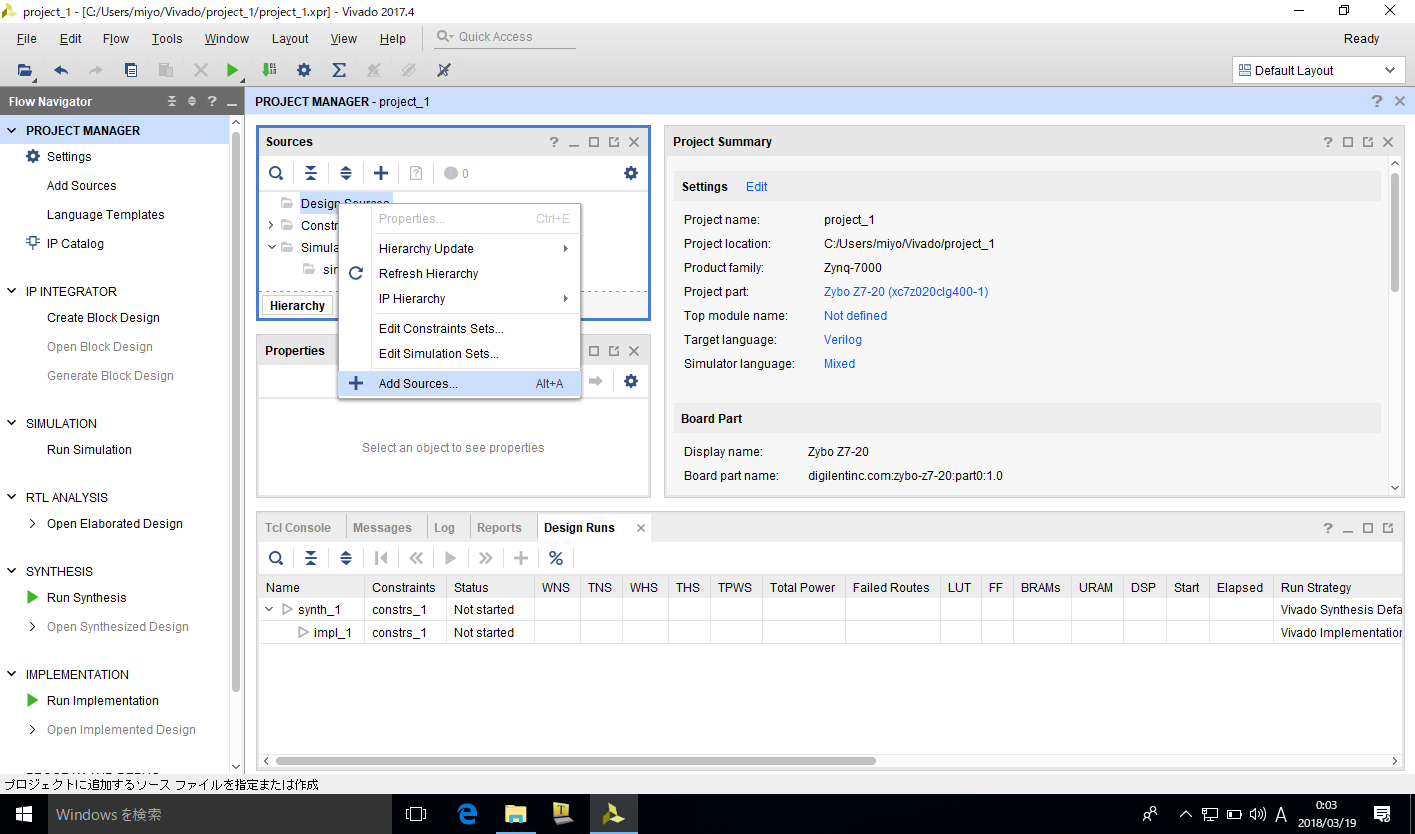
\includegraphics[width=.8\textwidth]{chapter03_figures/VirtualBox_Windows10_19_03_2018_00_03_27.png}
  \end{center}
  \caption{SourcesのDesign Sourceの上で右クリックし,Add Sources...を選択する}
 \end{figure}

 \begin{figure}[H]
  \begin{center}
   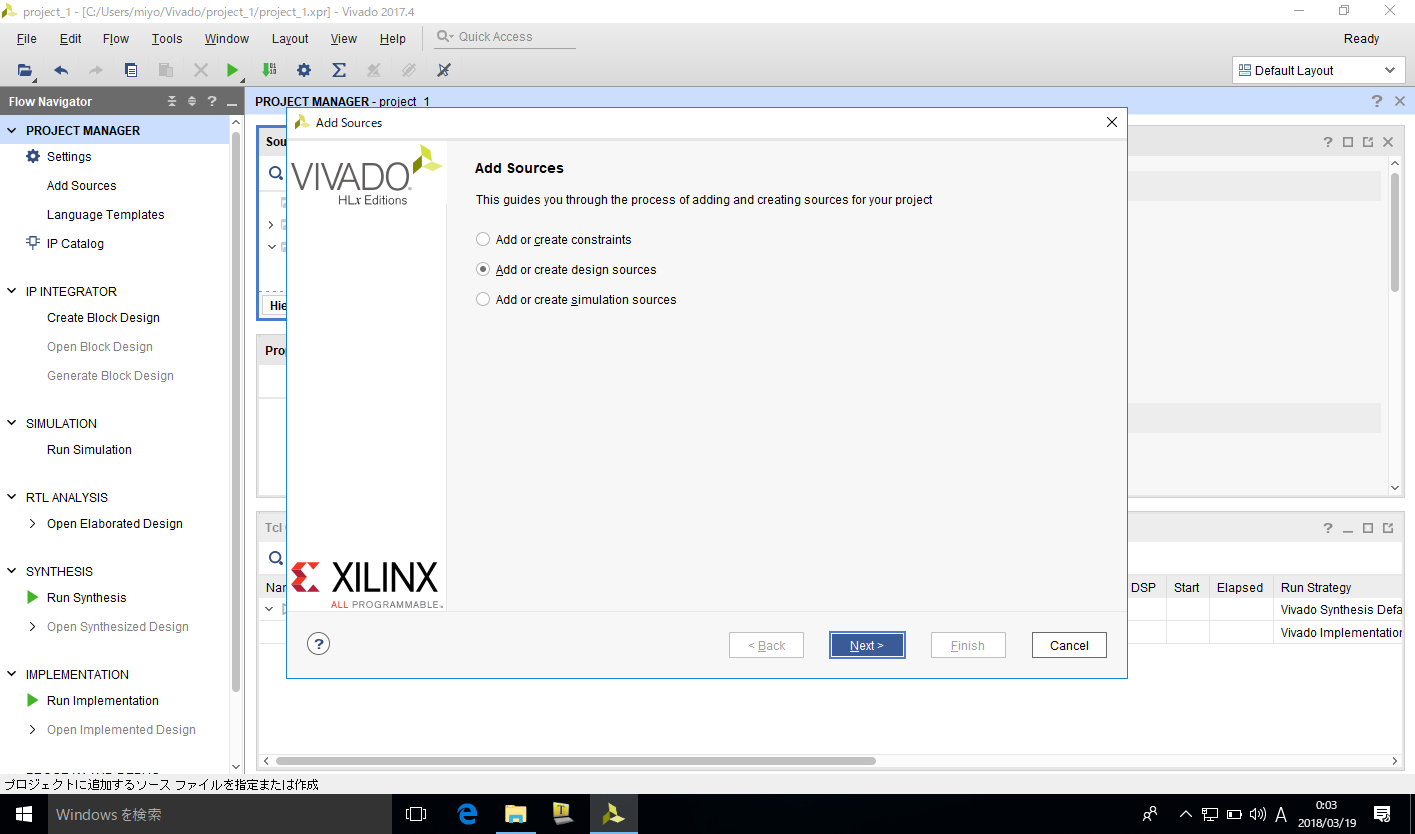
\includegraphics[width=.8\textwidth]{chapter03_figures/VirtualBox_Windows10_19_03_2018_00_03_35.png}
  \end{center}
  \caption{ファイル追加ダイアログが開く}
 \end{figure}

 \begin{figure}[H]
  \begin{center}
   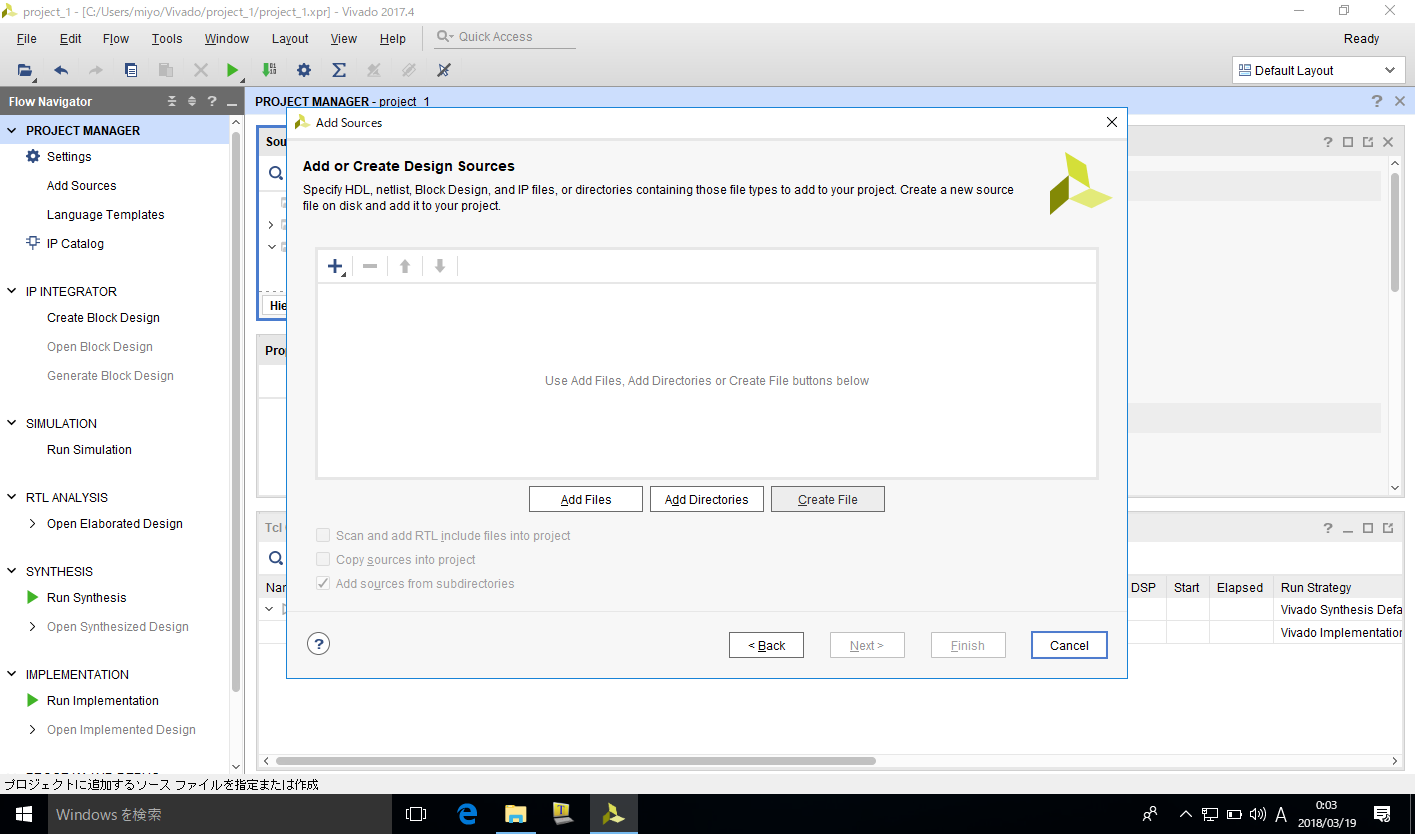
\includegraphics[width=.8\textwidth]{chapter03_figures/VirtualBox_Windows10_19_03_2018_00_03_42.png}
  \end{center}
  \caption{2番目のAdd or create design sources...にチェックをいれてNext$\gt$をクリック}
 \end{figure}

 \begin{figure}[H]
  \begin{center}
   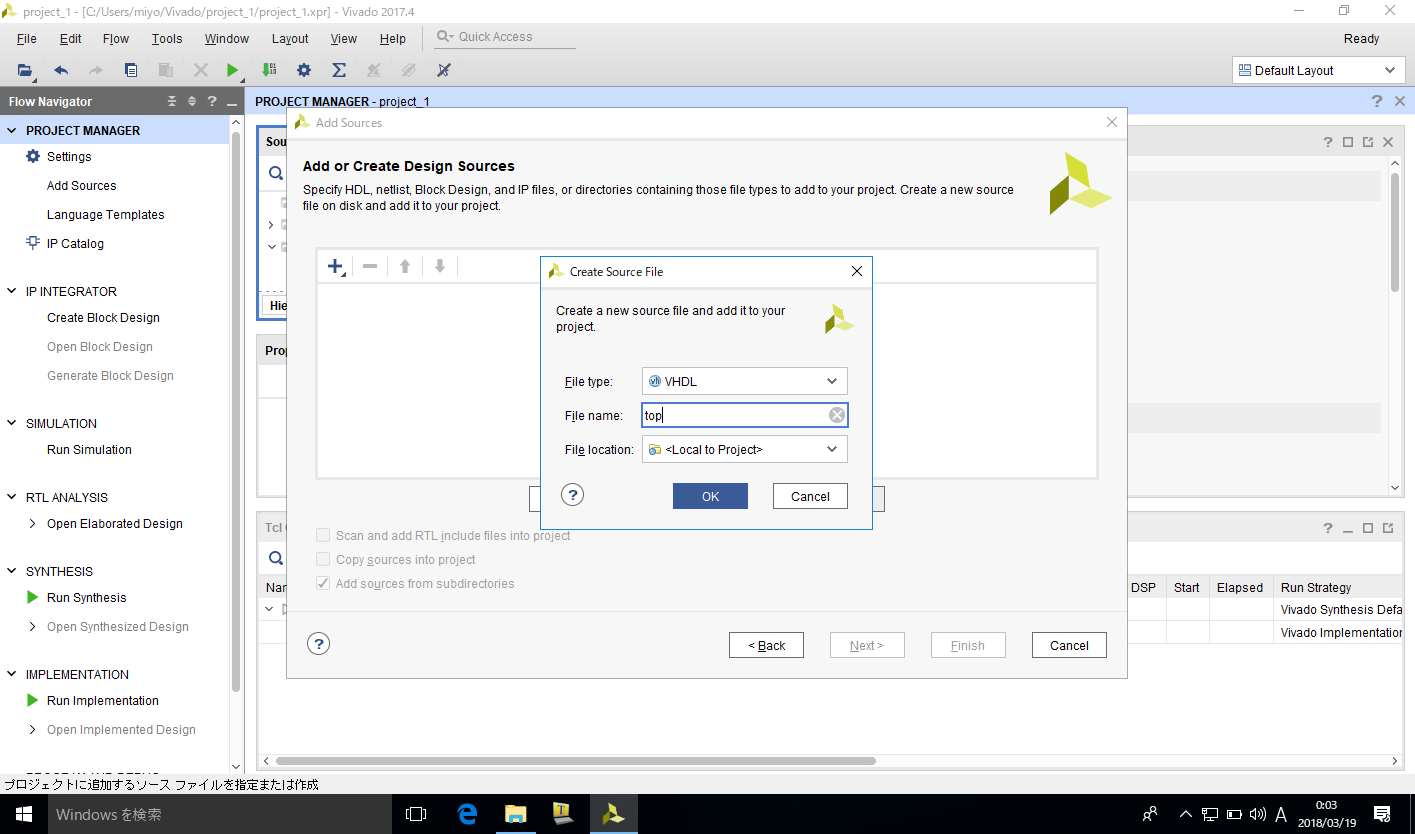
\includegraphics[width=.8\textwidth]{chapter03_figures/VirtualBox_Windows10_19_03_2018_00_03_54.png}
  \end{center}
  \caption{ここで新しくファイルを作るので,Create Fileをクリック}
 \end{figure}

 \begin{figure}[H]
  \begin{center}
   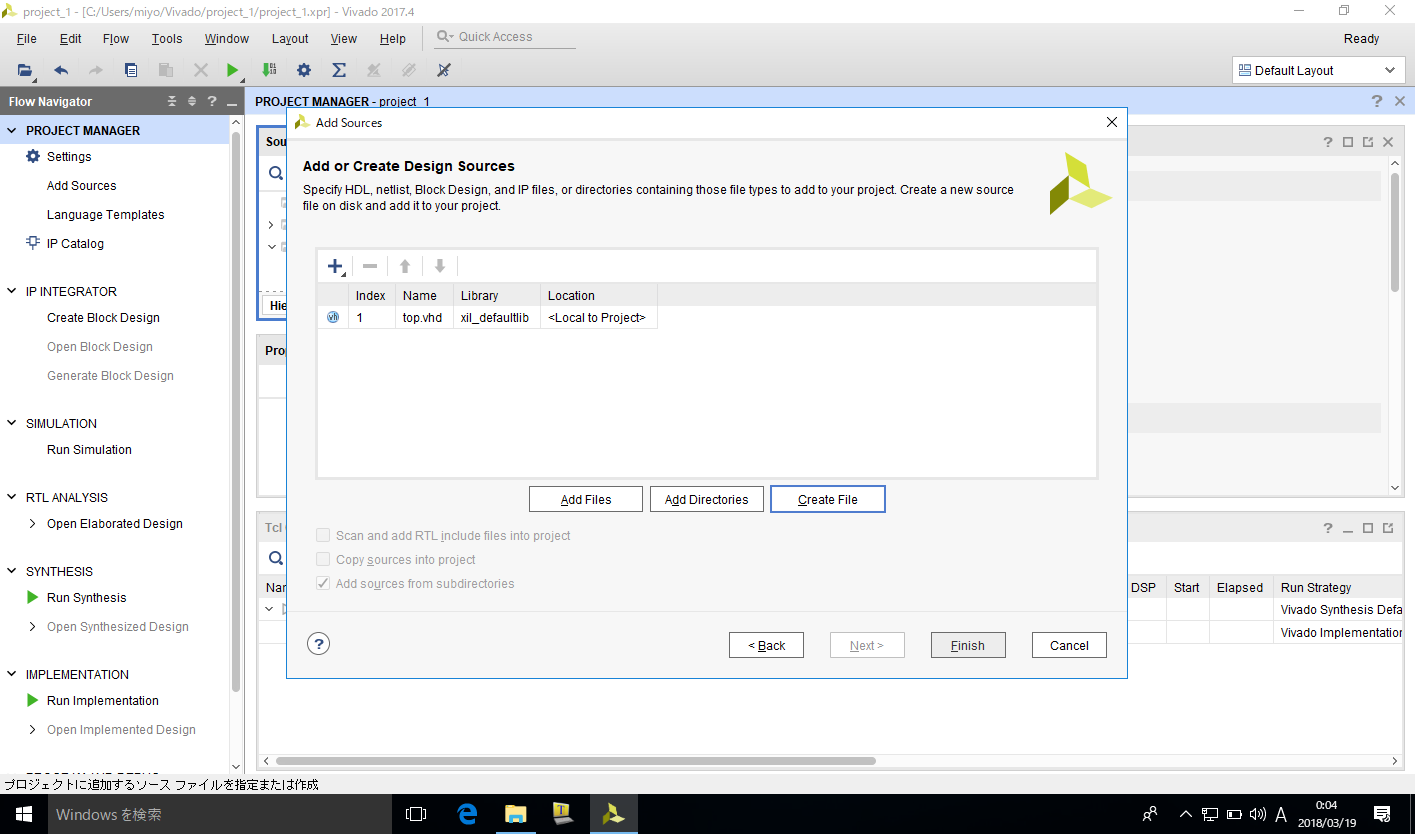
\includegraphics[width=.8\textwidth]{chapter03_figures/VirtualBox_Windows10_19_03_2018_00_04_01.png}
  \end{center}
  \caption{使用言語とモジュール名を決めます.ここではVHDLを使うこととし,名前をtopと決めてOKをクリック}
 \end{figure}

 \begin{figure}[H]
  \begin{center}
   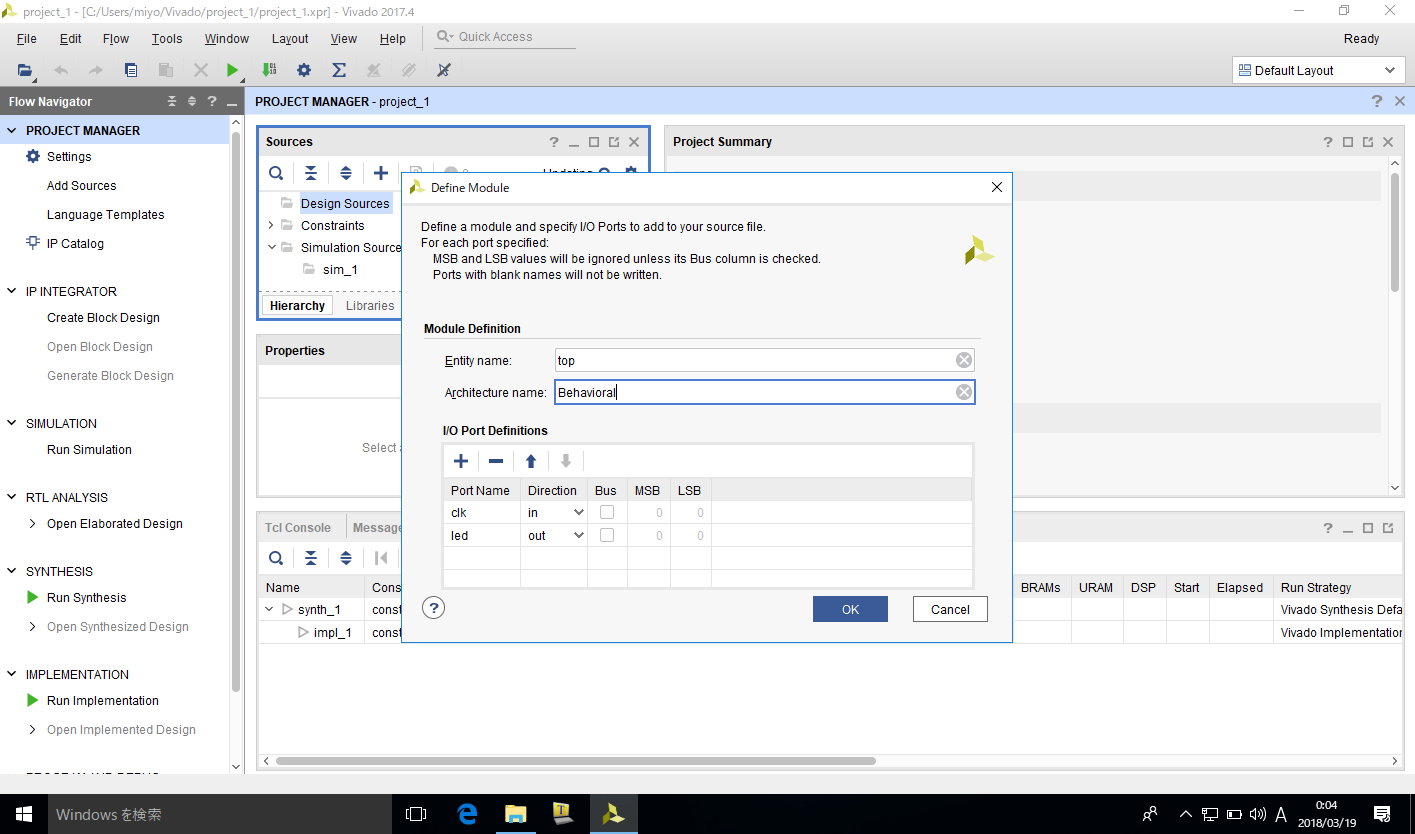
\includegraphics[width=.8\textwidth]{chapter03_figures/VirtualBox_Windows10_19_03_2018_00_04_44.png}
  \end{center}
  \caption{作成するファイルがリストに登録されたので,Finishをクリックします}
 \end{figure}

 \begin{figure}[H]
  \begin{center}
   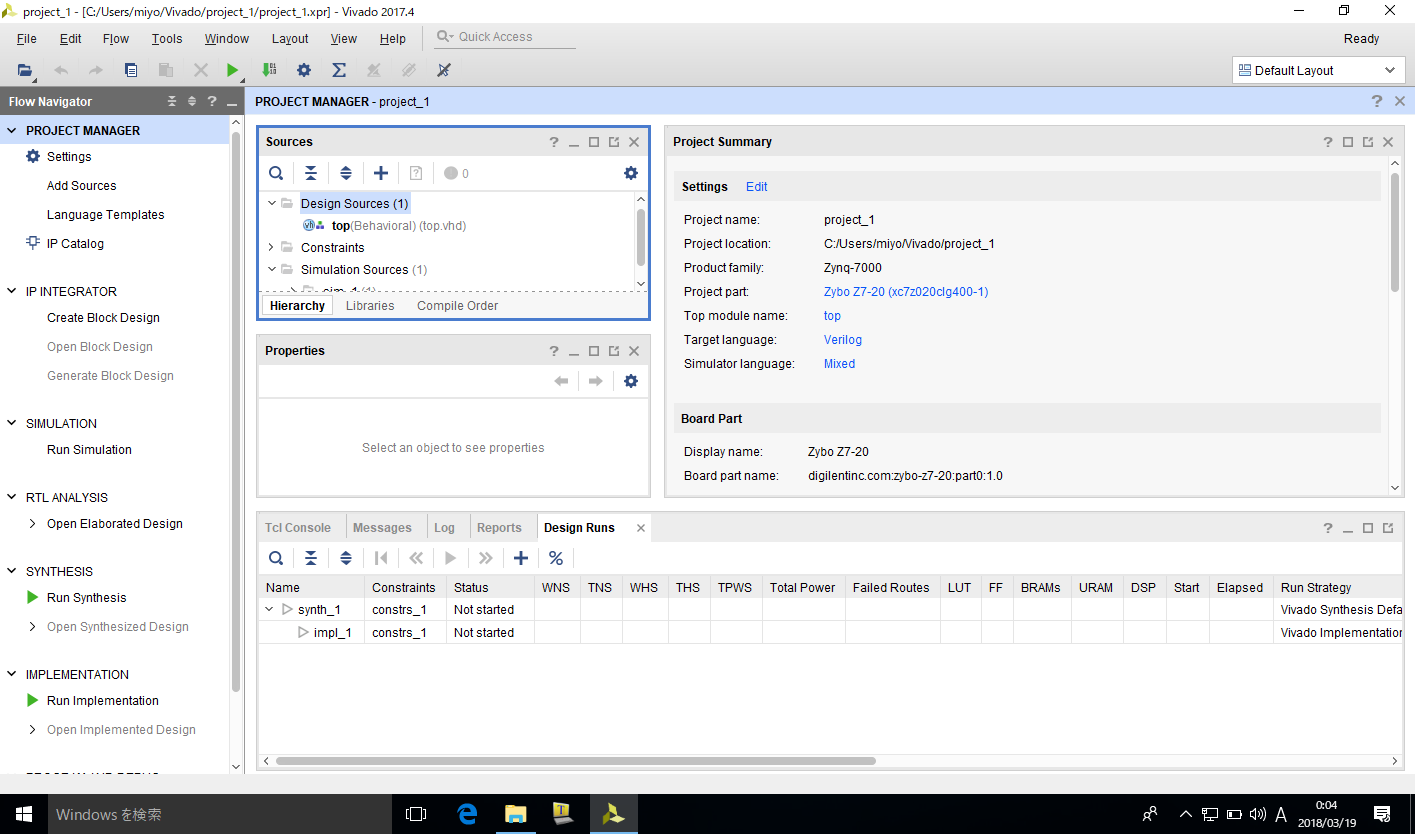
\includegraphics[width=.8\textwidth]{chapter03_figures/VirtualBox_Windows10_19_03_2018_00_04_59.png}
  \end{center}
  \caption{新たに作成したtopモジュールのポートなどを定義することができます.あとで自分で書いてもいいのですが,入力ポートのclkと出力ポートのledを追加しましょう.OKをクリックします}
 \end{figure}

 \begin{figure}[H]
  \begin{center}
   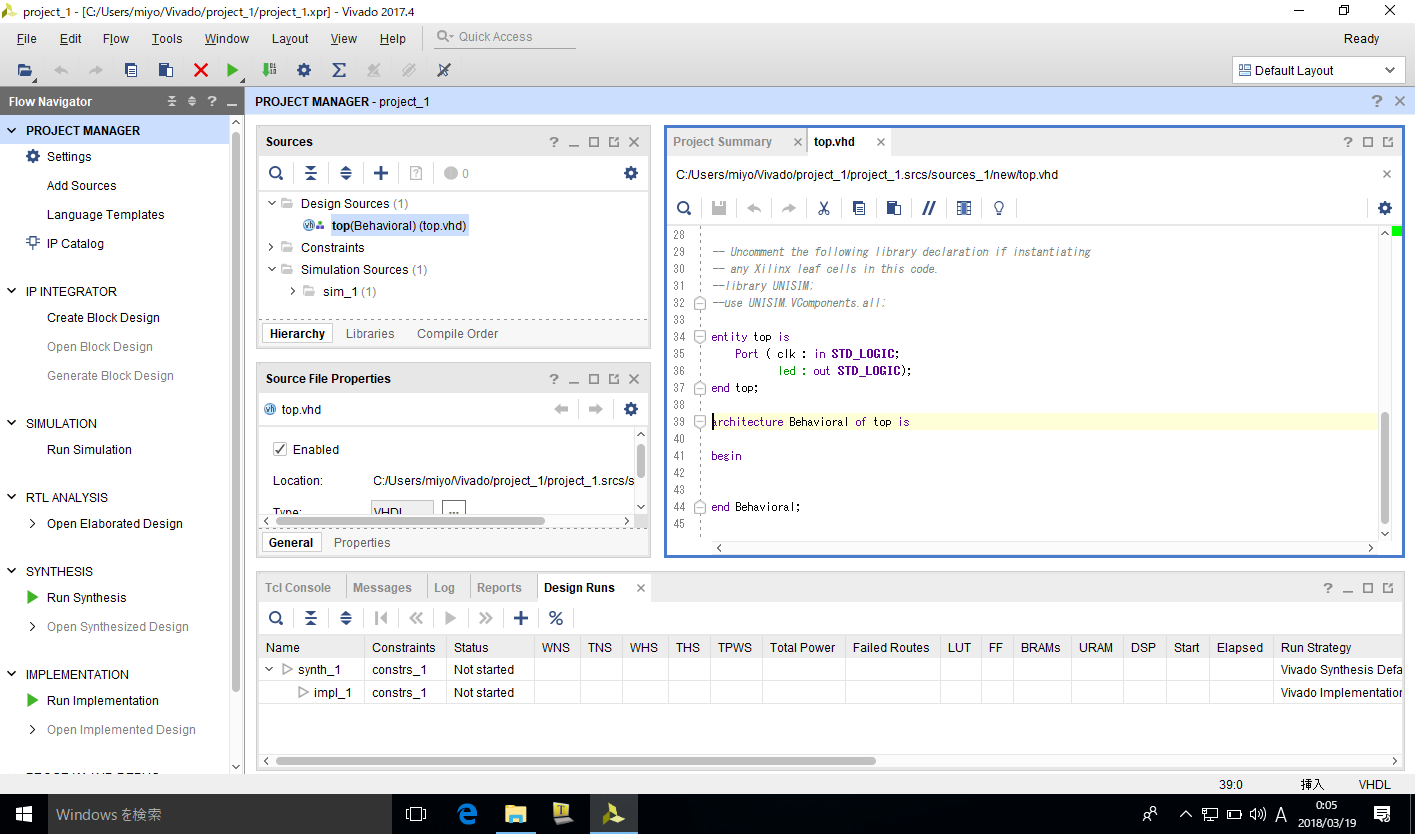
\includegraphics[width=.8\textwidth]{chapter03_figures/VirtualBox_Windows10_19_03_2018_00_05_13.png}
  \end{center}
  \caption{作成したtopモジュールがプロジェクトに組み込まれました}
 \end{figure}

 \begin{figure}[H]
  \begin{center}
   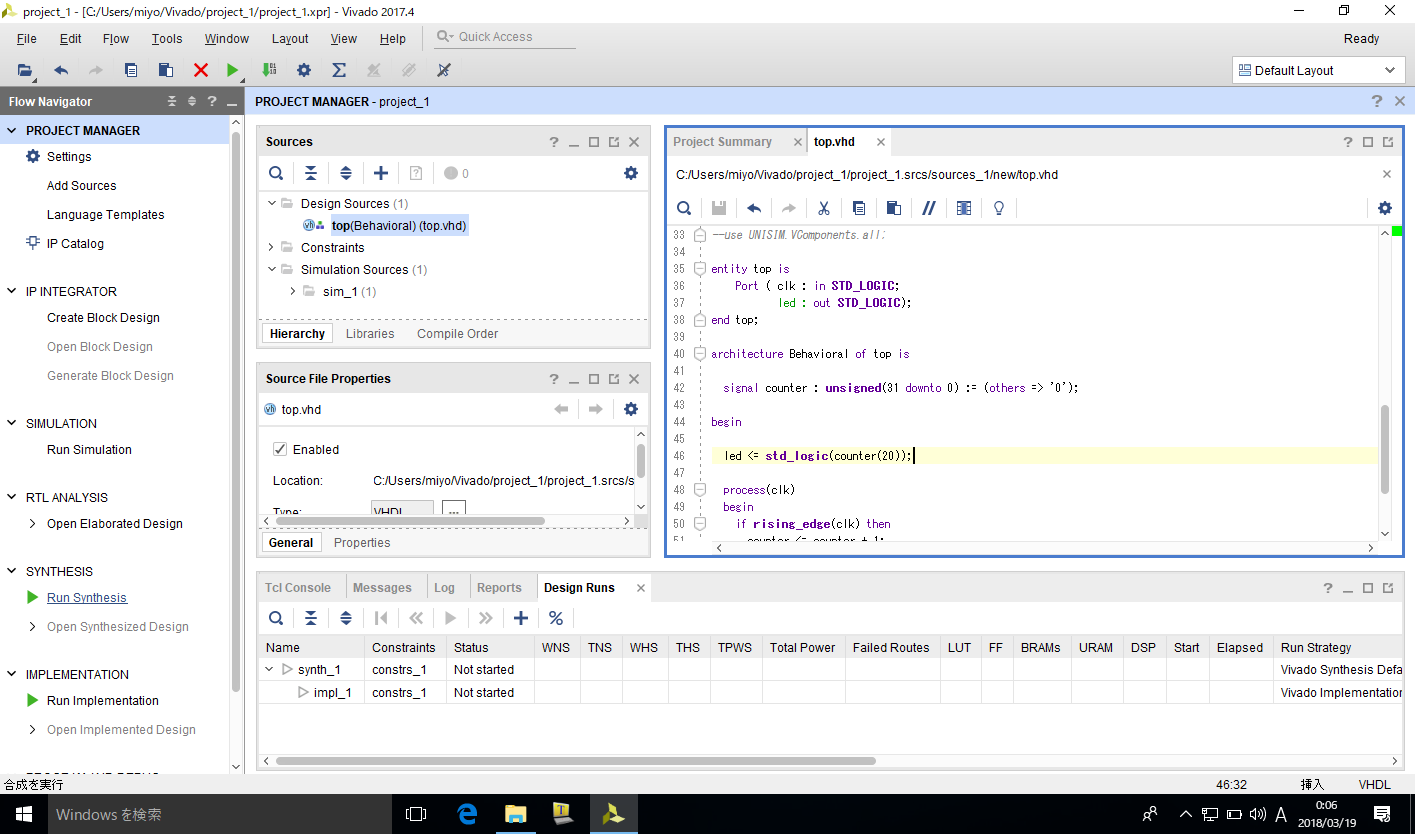
\includegraphics[width=.8\textwidth]{chapter03_figures/VirtualBox_Windows10_19_03_2018_00_06_55.png}
  \end{center}
  \caption{組み込まれたtopをダブルクリックするとファイルを編集することができます}
 \end{figure}

\subsection{デザインの修正}
ウィザードで作成したtopモジュールは雛形でしかないので,このままでは,もちろん所望の動作はしません.次の内容で書き変えてください.スペースの都合上,作成されたコメントは取り除いています.ファイルを編集するときには気をつけてください.また,リスト中のコメントは説明上のものですので,実際には入力する必要はありません.

\begin{figure}[H]
\begin{quote}
\begin{Verbatim}[frame=single, numbers=left, baselinestretch=0.8]
library IEEE;
use IEEE.STD_LOGIC_1164.ALL;
use ieee.numeric_std.all; -- 追加する.数値演算に必要(1).

entity top is
  Port ( clk : in STD_LOGIC;
         led : out STD_LOGIC); -- このPortはウィザードで作成された
end top;

architecture Behavioral of top is

  -- 次の行を追加.カウンタ変数の定義(2).
  signal counter : unsigned(31 downto 0) := (others => '0'); 

  begin
  -- 追加,ここから(3)
  led <= std_logic(counter(23)); -- カウンタの23bit目をledに接続

  process(clk) -- クロックの変化で動作するプロセス
  begin
    if rising_edge(clk) then -- クロックの立ち上がりであれば
      counter <= counter + 1; -- カウンタをインクリメント
    end if;
  end process;
  -- 追加,ここまで
end Behavioral;
  \end{Verbatim}
 \end{quote}
\end{figure}

追加箇所は多くないので,少し詳しくみてみましょう.

\paragraph{追加箇所(1)}
数値演算に必要なライブラリ,今回の場合でいうと``+''演算を利用するために\verb|use ieee.numeric_std.all|という前置きをしています.

\paragraph{追加箇所(2)}
LEDチカチカの,``チカチカ''というタイミングを制御するためのカウンタ変数を定義です.+演算を利用したいので\verb|unsigned|型で定義しています.

\paragraph{追加箇所(3)}
いわば処理の本体です.一行目の代入文は,定義したcounter変数の23bit目を出力ポートであるledに接続することを意味しています.\verb|unsigned|の1bitですので\verb|std_logic|に型変換しています.次のprocess文では,clkが立ち上がることにcounterに1を足すことを意味しています.すなわち,(3)で追加した部分では,clkの立ち上がり8M回毎にledの'1'と'0'が反転する回路を定義していることになります.


\subsection{まずは合成してみる}
ファイルの編集がおわったら合成してみましょう.といっても,左サイドにあるFlow Navigatorの中にあるRun Synthesisをクリックするだけです.

 \begin{figure}[H]
  \begin{center}
   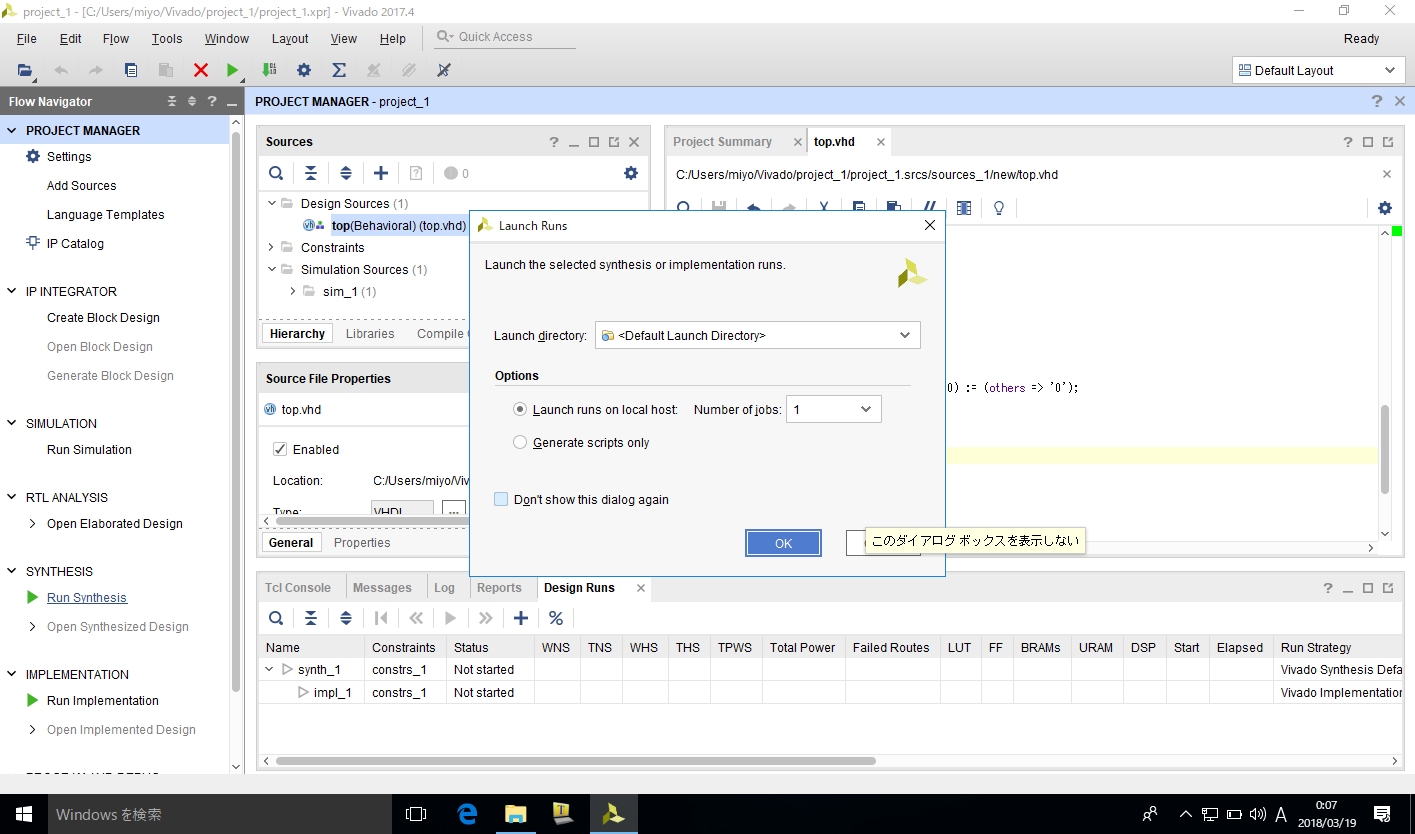
\includegraphics[width=.8\textwidth]{chapter03_figures/VirtualBox_Windows10_19_03_2018_00_07_02.png}
  \end{center}
  \caption{Run Synthesisをクリックすると合成開始ダイアログが開く.OKをクリックして合成を開始}
 \end{figure}

 \begin{figure}[H]
  \begin{center}
   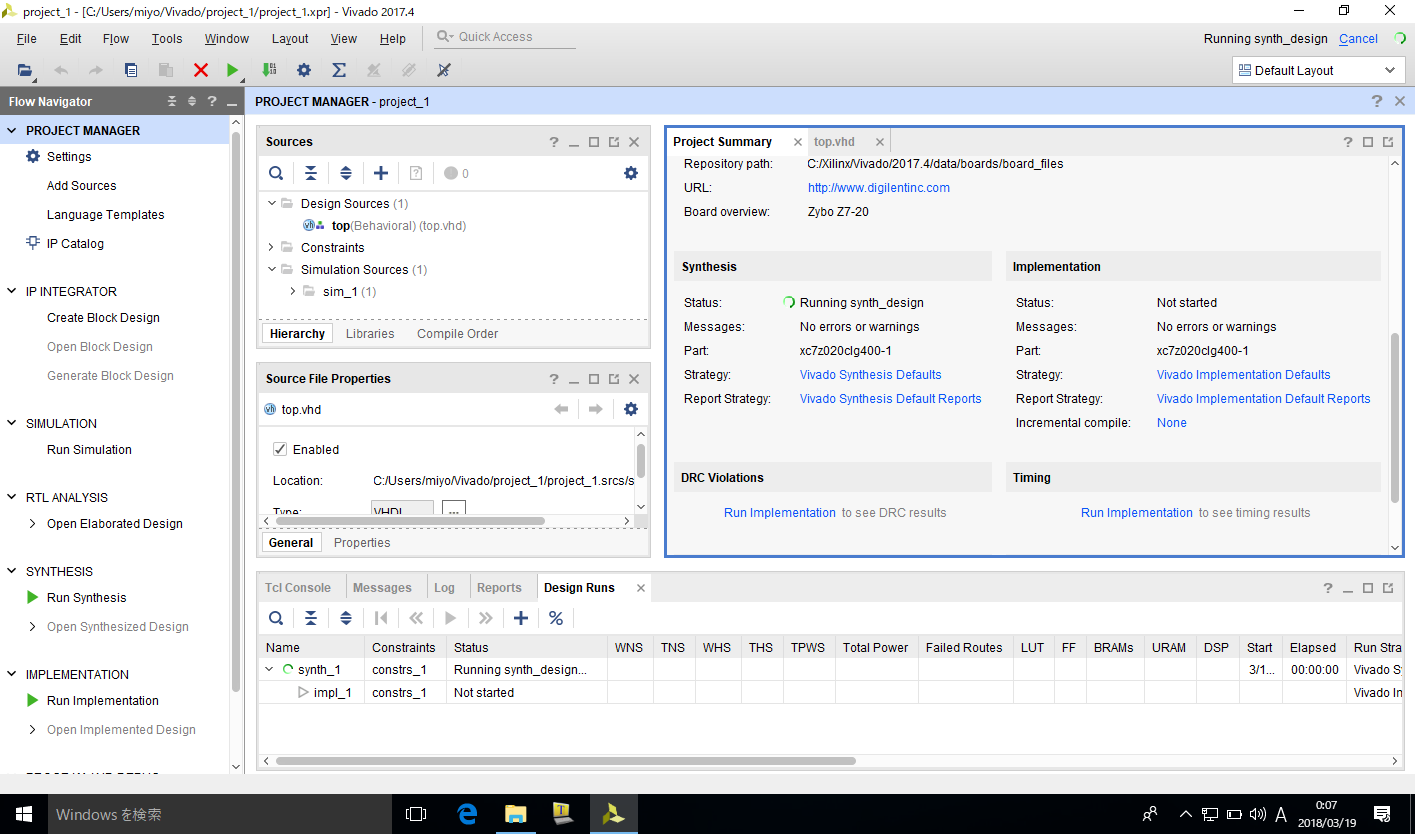
\includegraphics[width=.8\textwidth]{chapter03_figures/VirtualBox_Windows10_19_03_2018_00_07_16.png}
  \end{center}
  \caption{合成中は,Running Synth\_designの横に,ぐるぐるアニメーションが表示される}
 \end{figure}

 \begin{figure}[H]
  \begin{center}
   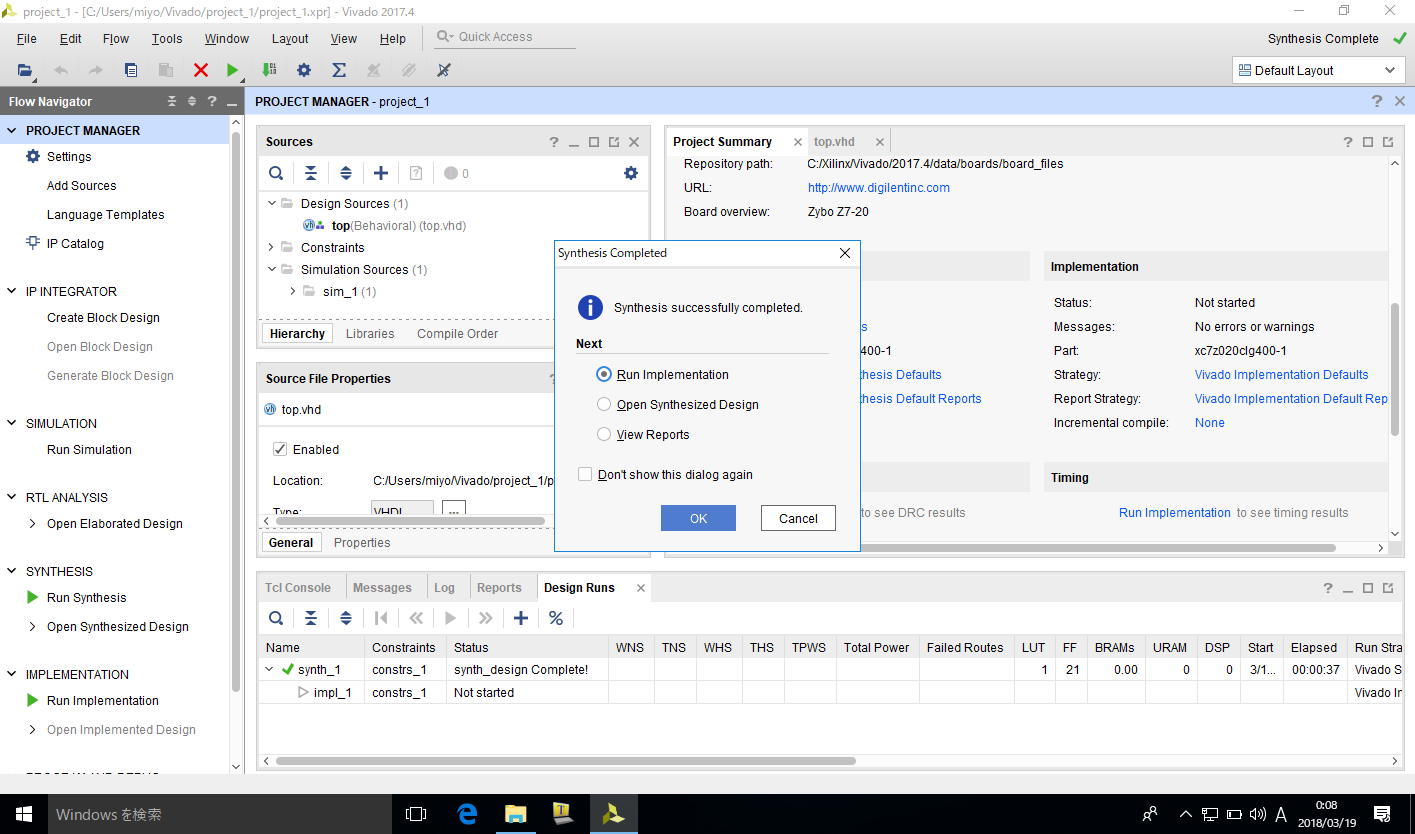
\includegraphics[width=.8\textwidth]{chapter03_figures/VirtualBox_Windows10_19_03_2018_00_08_08.png}
  \end{center}
  \caption{合成が完了した}
 \end{figure}

\subsection{I/Oの設定}
合成が完了したことでデザインがVivadoに受け付けられることが確認できました.しかし,これでそのままFPGAでデザインが動くわけではありません.I/Oピンの設定をしていないからです.HDLのデザイン上は,入力ポートclkと出力ポートのledを定義しましたが,Vivadoは,このポートをFPGAのどのピンに割り当てていいか分かりません.FPGAを使った開発では人手でこの割り当てを決める必要があります.

ピンの割当ては合成結果を下敷にGUIで行なうことができます.まずは,合成結果を表示します.

 \begin{figure}[H]
  \begin{center}
   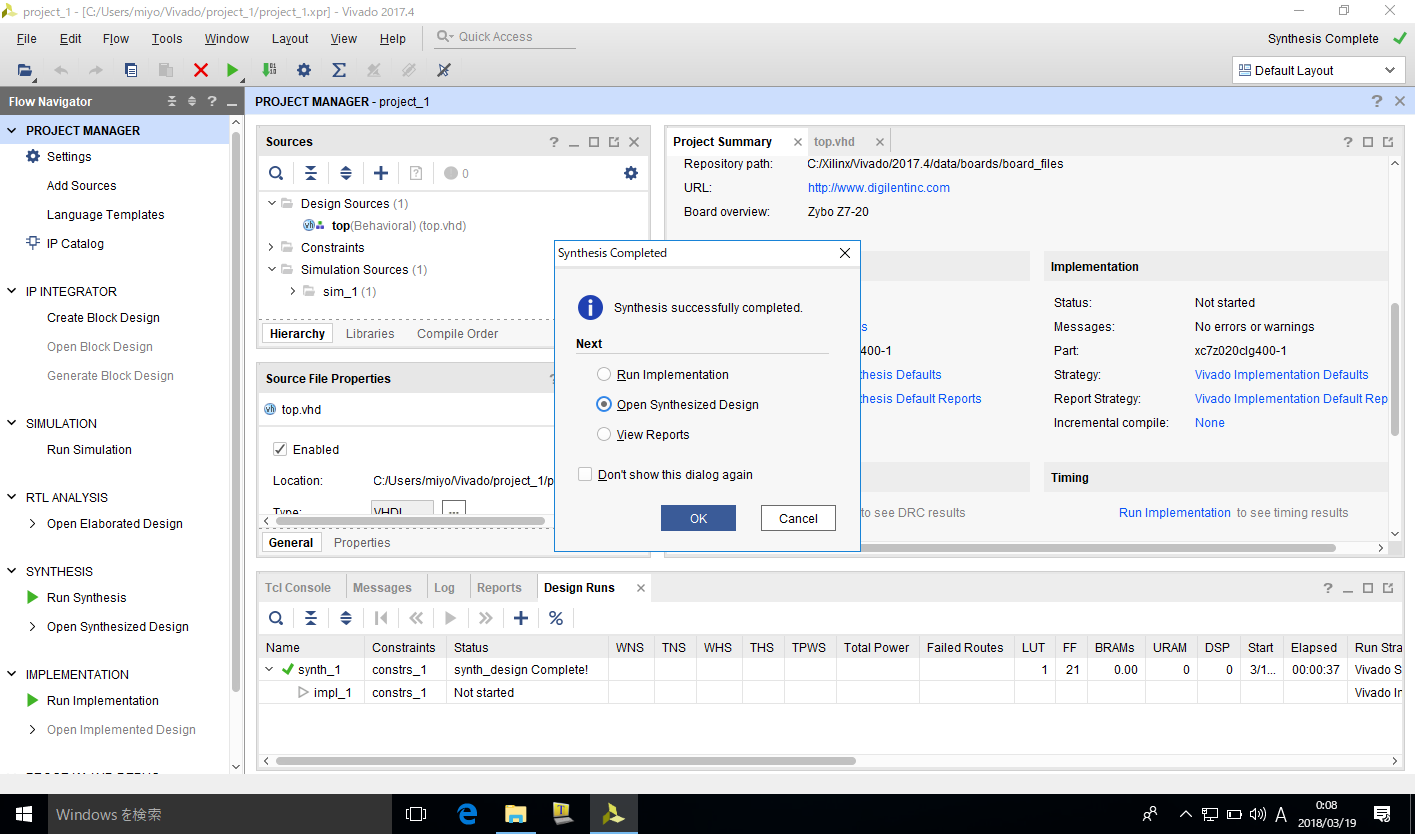
\includegraphics[width=.8\textwidth]{chapter03_figures/VirtualBox_Windows10_19_03_2018_00_08_14.png}
  \end{center}
  \caption{合成後のダイアログで,``Open Synthesized Design''を選択し,OKをクリックする}
 \end{figure}

もし,うっかり合成後のダイアログを閉じてしまったり,ピン配置を指定しないまま次のステップにすすんでしまった場合には,Flow Navigatorの中にあるOpen Synthesized Designをクリックしましょう.

合成結果が表示できたら,LayoutのI/O PlanningをクリックしてI/O設定用のモードに変更します.
 \begin{figure}[H]
  \begin{center}
   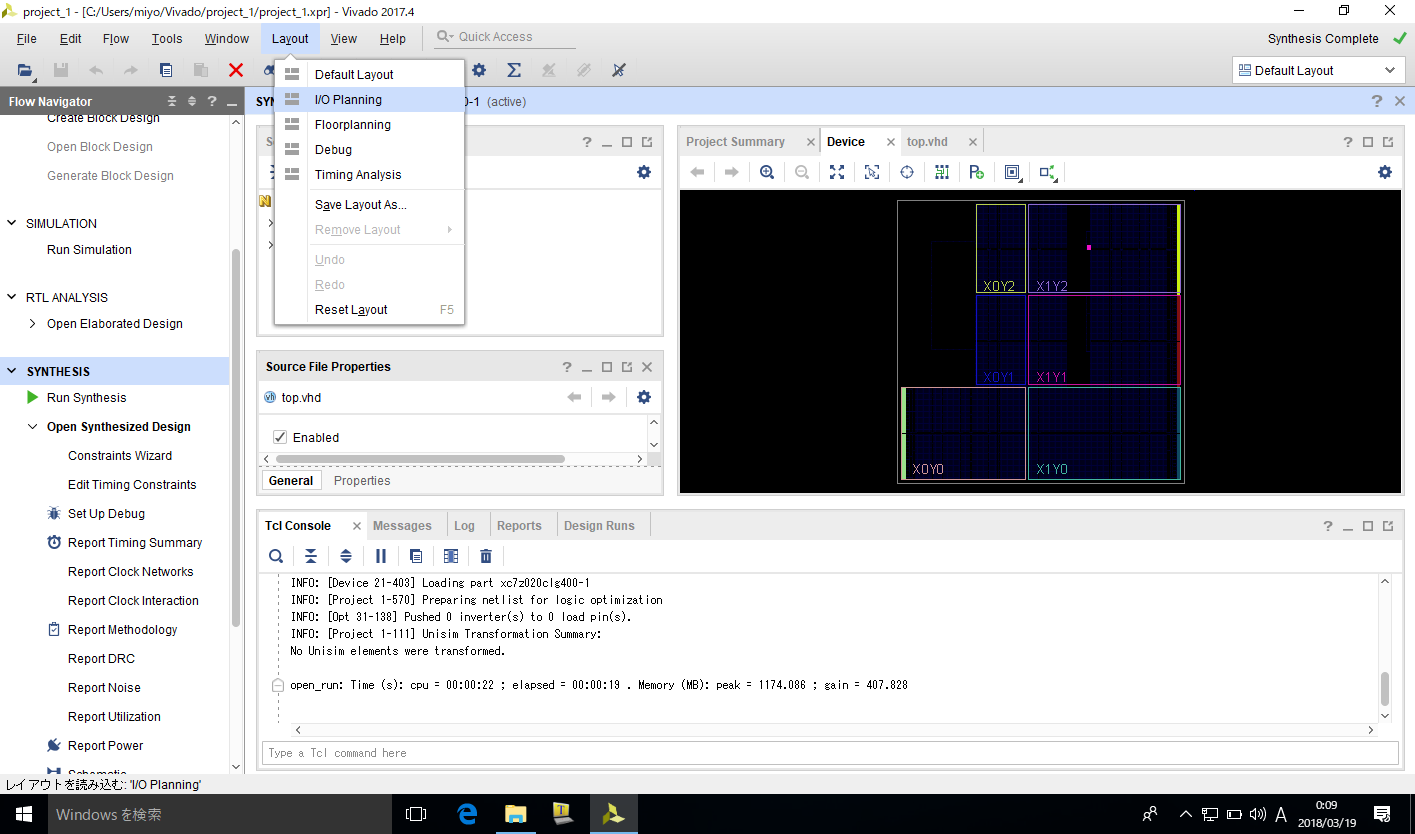
\includegraphics[width=.8\textwidth]{chapter03_figures/VirtualBox_Windows10_19_03_2018_00_09_32.png}
  \end{center}
  \caption{LayoutのI/O PlanningをクリックしてI/O設定用のモードに変更}
 \end{figure}

画面下のI/O割当て表でピン配置を決定します.clkとledのPackage pinを,それぞれ,K17とM14に決め,どちらもI/O stdをLVCMOS33を選択します.
 \begin{figure}[H]
  \begin{center}
   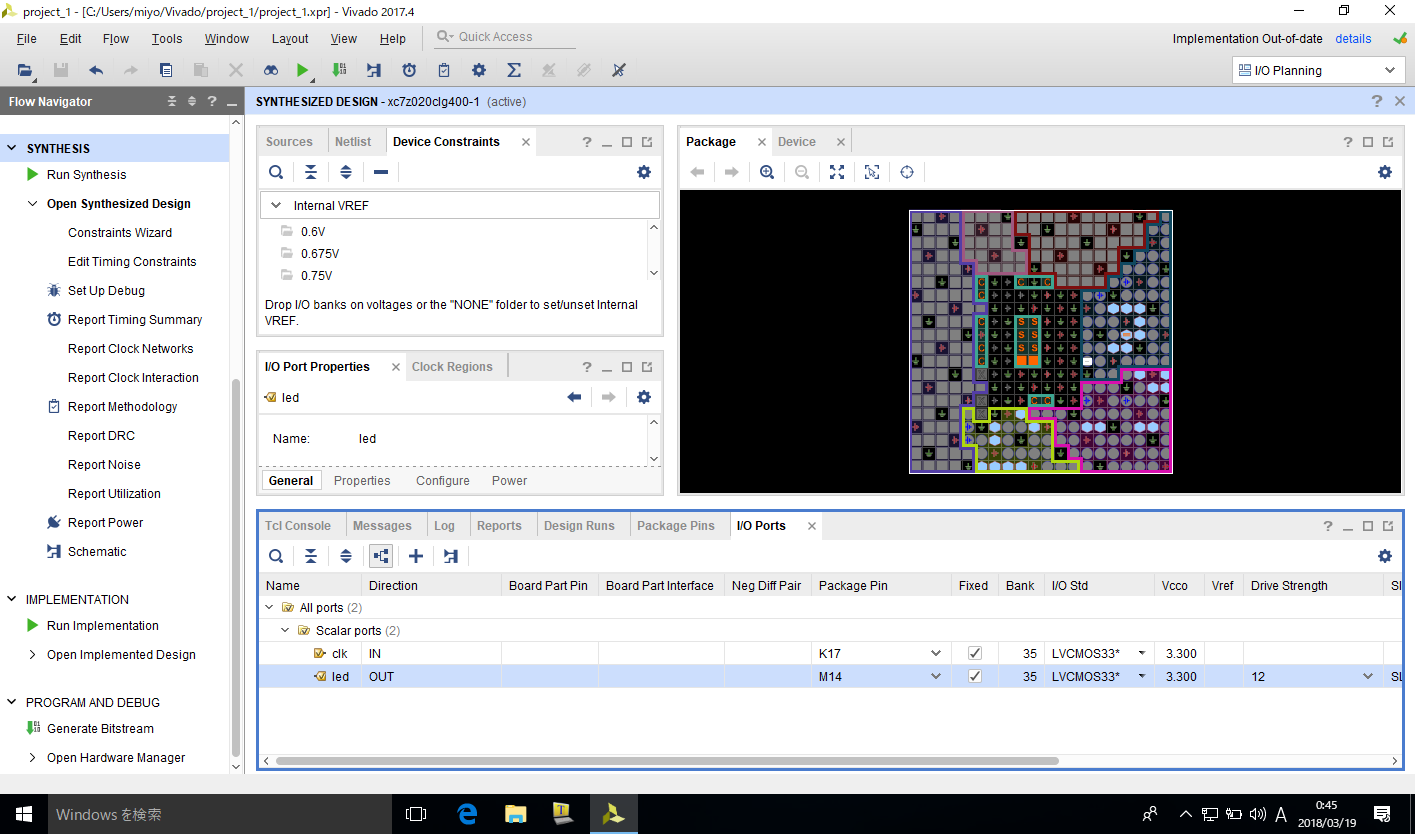
\includegraphics[width=.8\textwidth]{chapter03_figures/VirtualBox_Windows10_19_03_2018_00_45_27.png}
  \end{center}
  \caption{I/Oのピン割り当てを決める}
 \end{figure}

\subsection{合成・配置配線}
ピン配置がおわったので,FPGA向けの書き込みファイルを作成します.Flow Navigatorの中にあるGenerate bitstreamをクリックするだけです.

 \begin{figure}[H]
  \begin{center}
   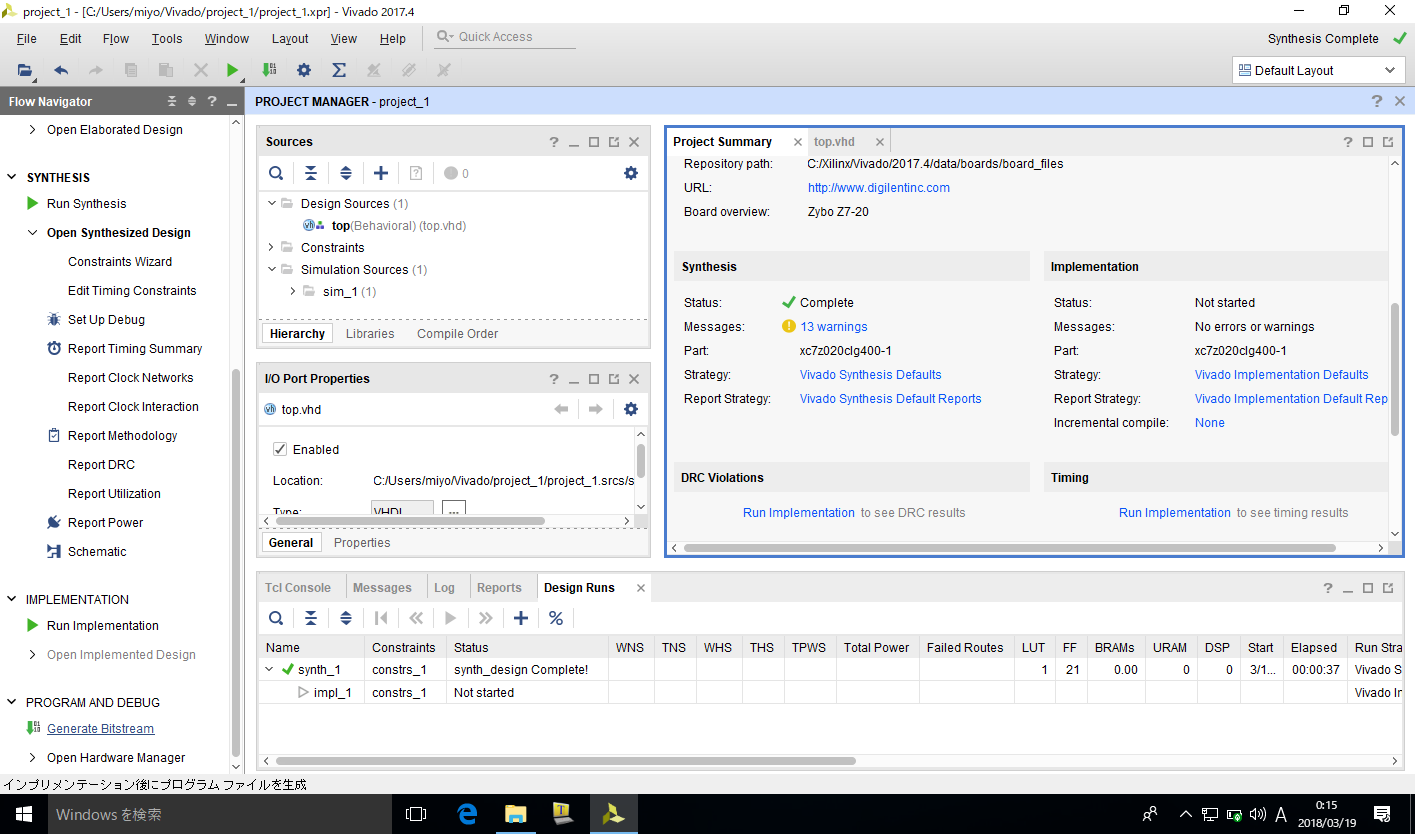
\includegraphics[width=.8\textwidth]{chapter03_figures/VirtualBox_Windows10_19_03_2018_00_15_52.png}
  \end{center}
  \caption{Flow Navigatorの中にあるGenerate bitstreamをクリックする.必要な合成・配置配線は一気通貫に実行される \label{fig:file_save_dialog}}
 \end{figure}

\subsubsection{制約ファイルの保存}
おそらく先のピン配置の変更が保存されていないので,図\ref{fig:file_save_dialog}のダイアログが開くことでしょう.もちろん保存してください.

 \begin{figure}[H]
  \begin{center}
   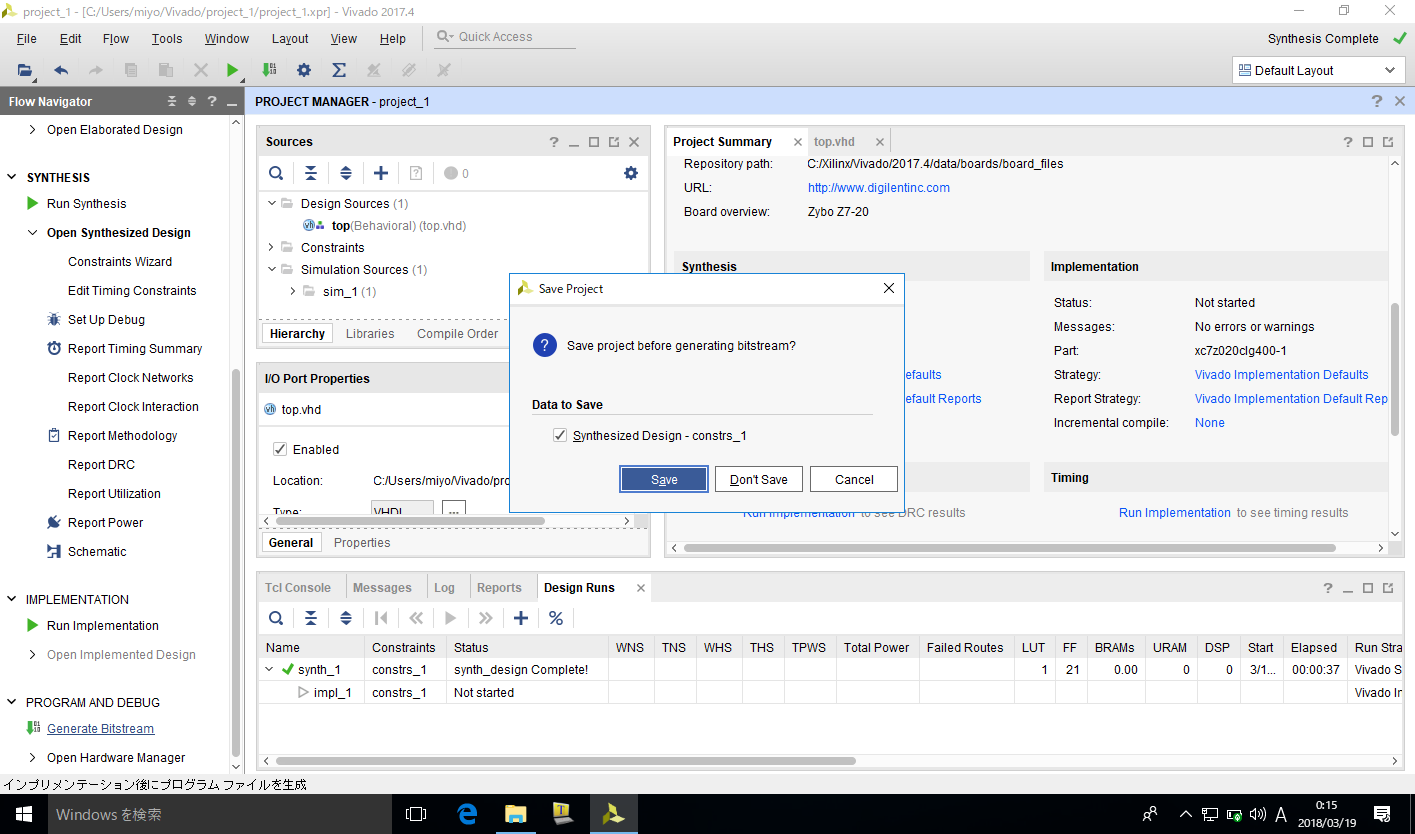
\includegraphics[width=.8\textwidth]{chapter03_figures/VirtualBox_Windows10_19_03_2018_00_15_59.png}
  \end{center}
  \caption{ピン配置の変更が保存されてないために表示されるダイアログ.Saveをクリック. \label{fig:file_save_dialog}}
 \end{figure}

 \begin{figure}[H]
  \begin{center}
   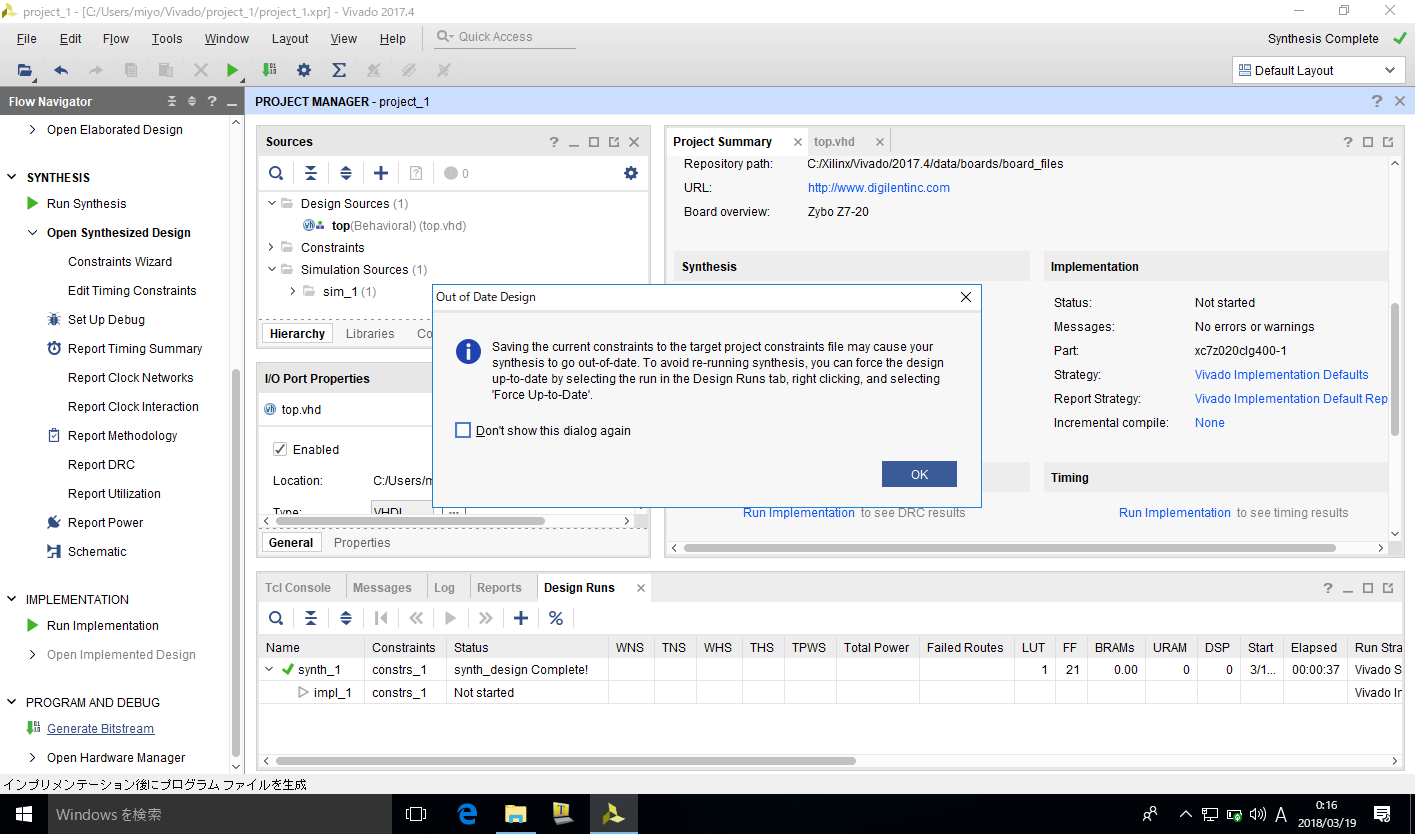
\includegraphics[width=.8\textwidth]{chapter03_figures/VirtualBox_Windows10_19_03_2018_00_16_26.png}
  \end{center}
  \caption{ファイル保存すると合成の結果が無効になるよという警告.OKで閉じる.}
 \end{figure}

\subsubsection{制約ファイルの指定(最初だけ)}
はじめは,保存先のファイルが用意されていないので,図\ref{fig:xdc_config}のダイアログが開きます.ここでは,HDLモジュールと同じ名前のtopというファイル名にします.なお,拡張子はxdcで自動的に付与されます.

 \begin{figure}[H]
  \begin{center}
   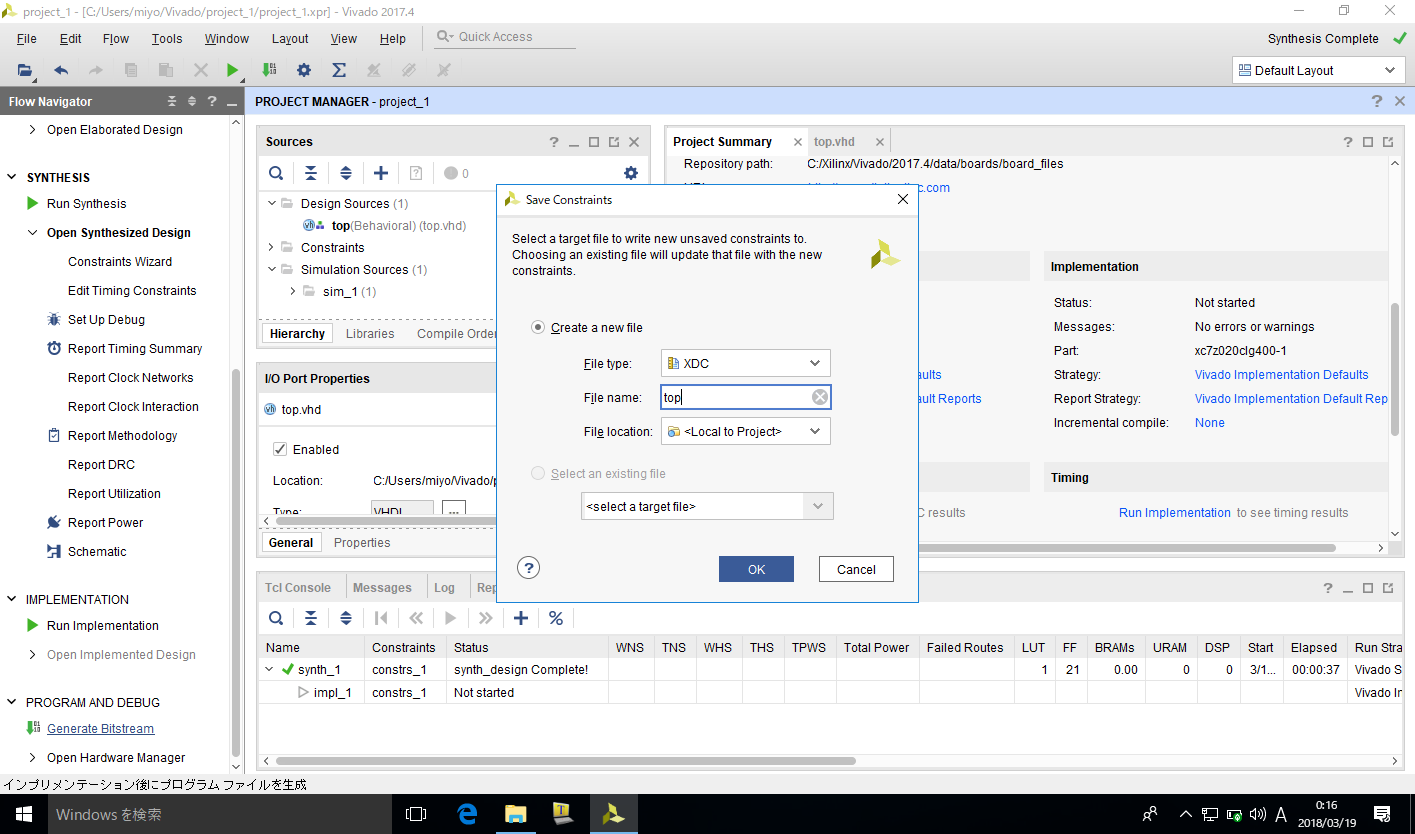
\includegraphics[width=.8\textwidth]{chapter03_figures/VirtualBox_Windows10_19_03_2018_00_16_35.png}
  \end{center}
  \caption{ピン配置を保存するファイルの作成を促すダイアログ.topという名前にしてOKをクリック \label{fig:xdc_config}}
 \end{figure}

\subsubsection{合成・配置配線の開始}
指定したピン配置の設定によって合成からやりなおしになります.``Yes''をクリックしてフローをすすめます.

 \begin{figure}[H]
  \begin{center}
   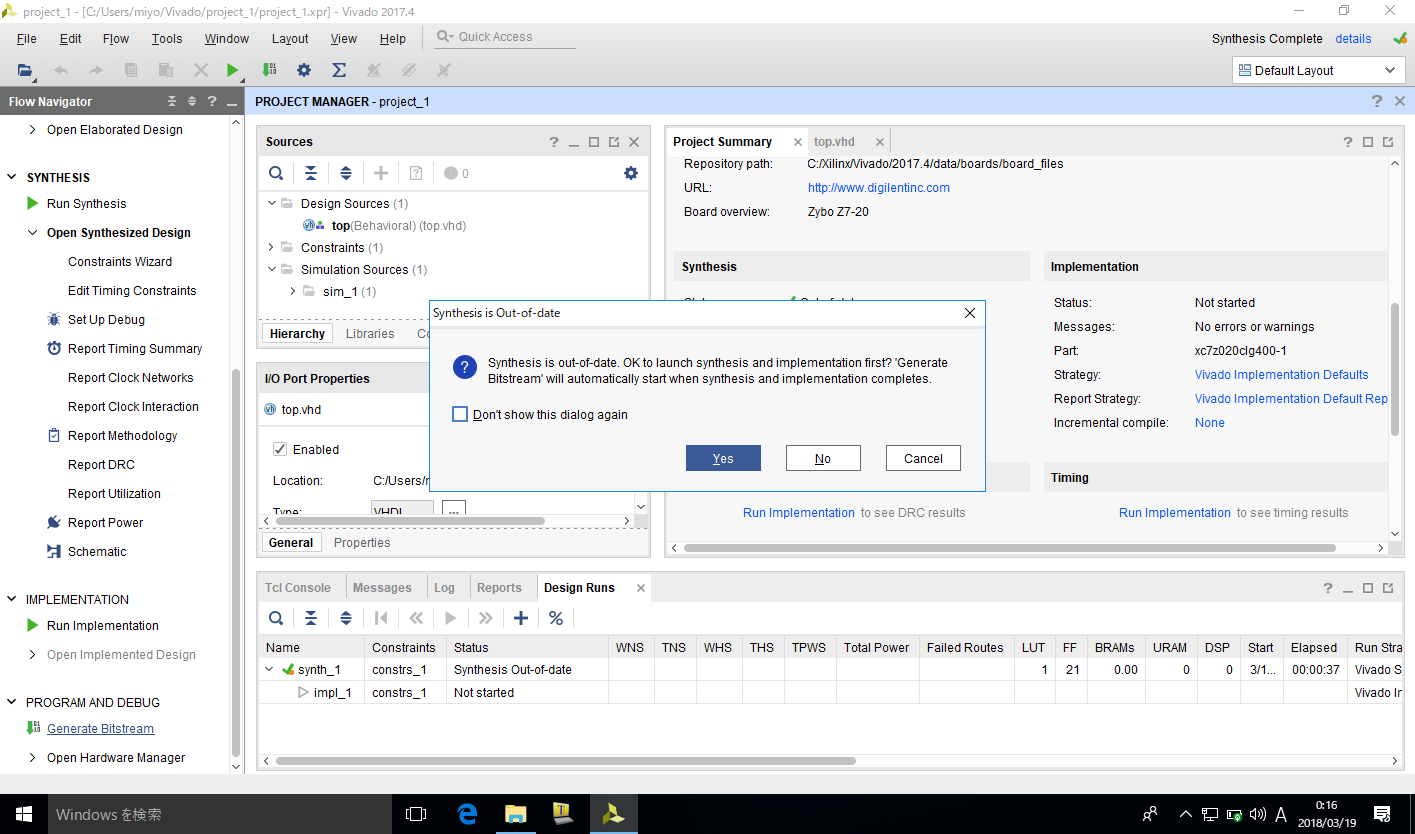
\includegraphics[width=.8\textwidth]{chapter03_figures/VirtualBox_Windows10_19_03_2018_00_16_41.png}
  \end{center}
  \caption{合成からやりなおし}
 \end{figure}

 \begin{figure}[H]
  \begin{center}
   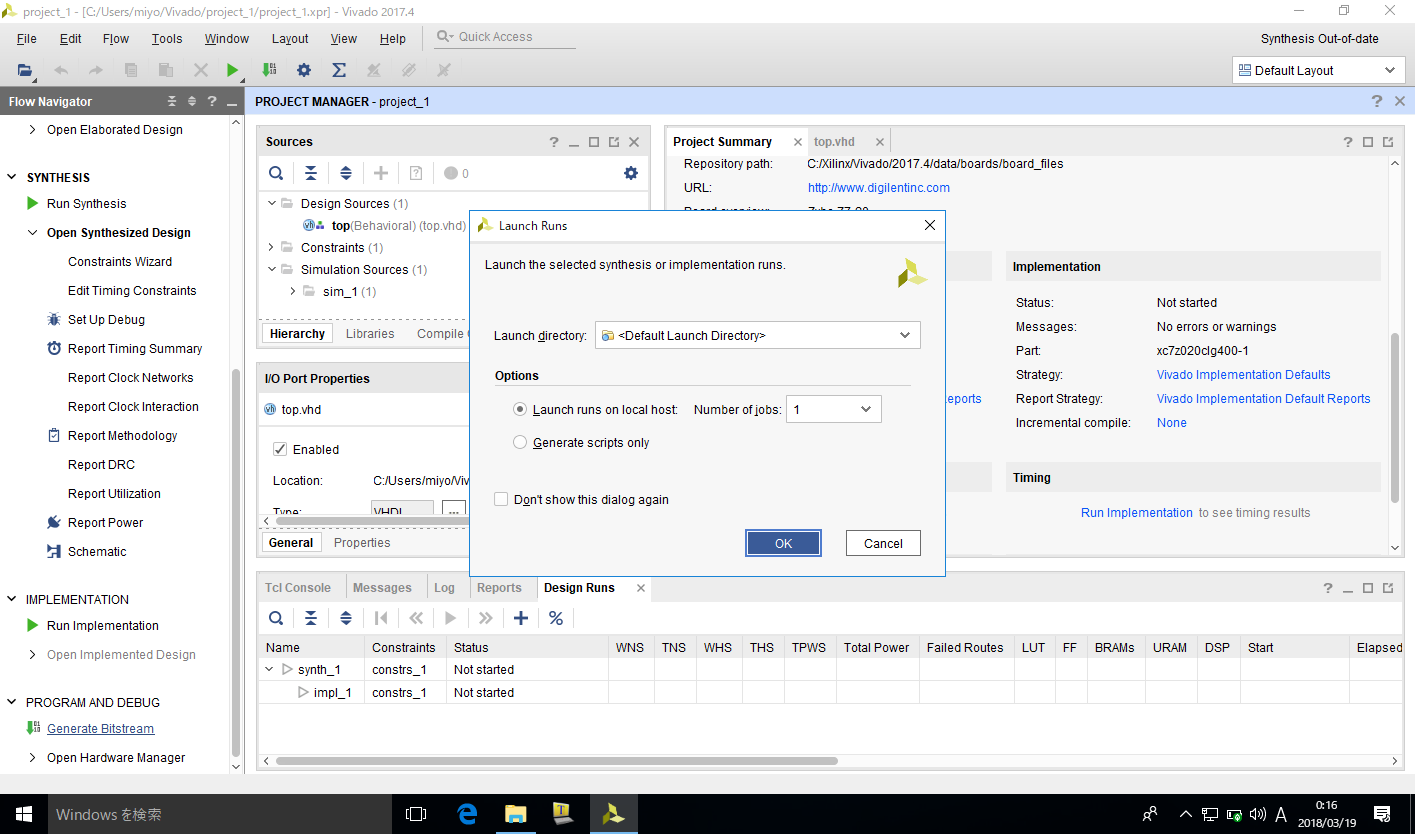
\includegraphics[width=.8\textwidth]{chapter03_figures/VirtualBox_Windows10_19_03_2018_00_16_46.png}
  \end{center}
  \caption{合成開始ダイアログ.OKで合成を開始.}
 \end{figure}

 \begin{figure}[H]
  \begin{center}
   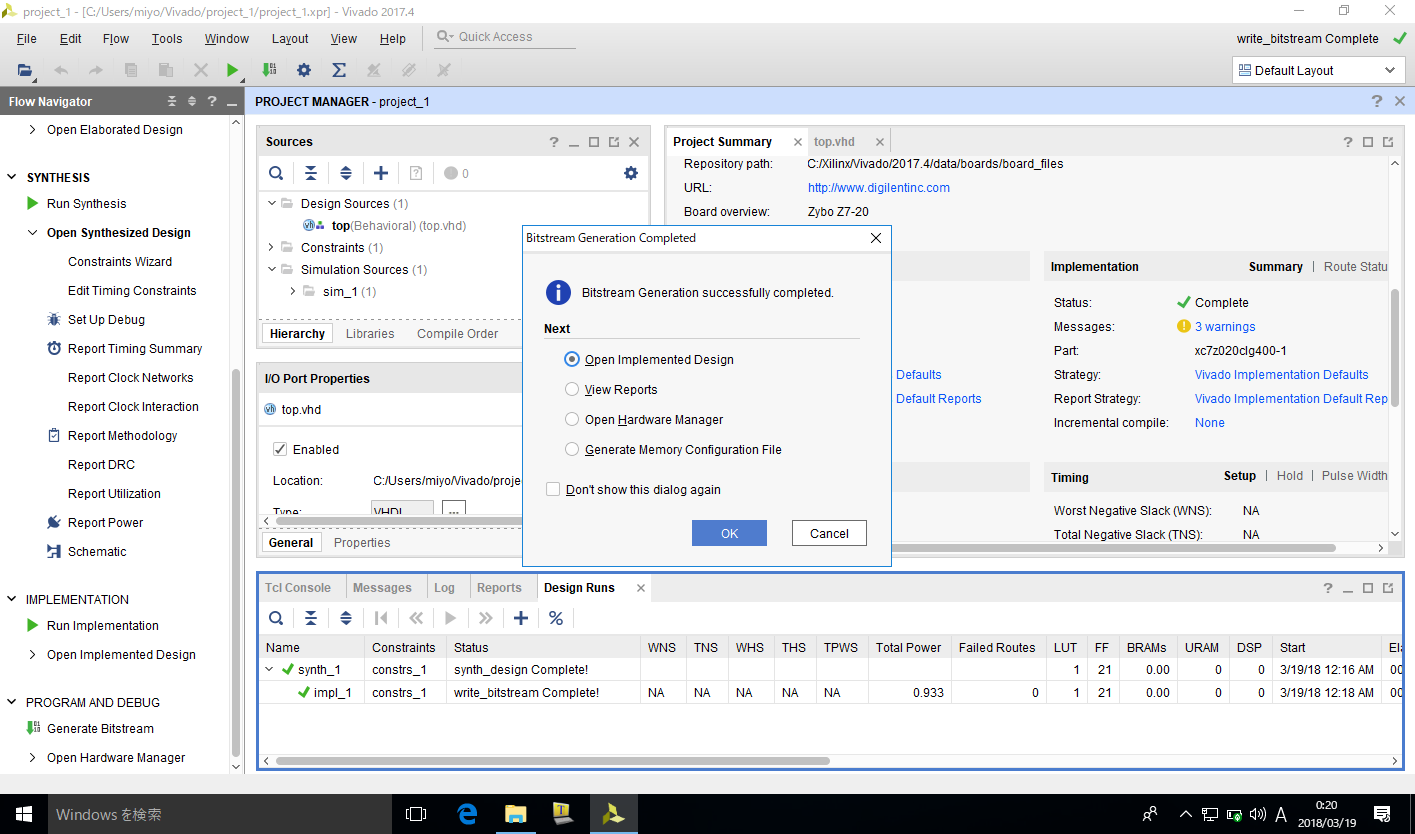
\includegraphics[width=.8\textwidth]{chapter03_figures/VirtualBox_Windows10_19_03_2018_00_20_45.png}
  \end{center}
  \caption{合成が無事に完了した.メインウインドウにCompleteという文字と緑のチェックマークがついている \label{fig:completed}}
 \end{figure}

\subsection{配置配線結果の確認}

配置配線後,どのようにFPGA上に回路が配置されたかを確認することができます.今回は指定していませんが,動作クロックの指定を行った場合などには,正しくクロックの指定ができているか,その指定にあった回路ができているか,を確認する必要があります.

今回は,まず雰囲気だけみてみましょう.合成後の図\ref{fig:completed}のダイアログで,Open Implementation DesignにチェックをいれてOKをクリックするか,Navigator FlowでOpen Implemnetation Designをクリックします.

 \begin{figure}[H]
  \begin{center}
   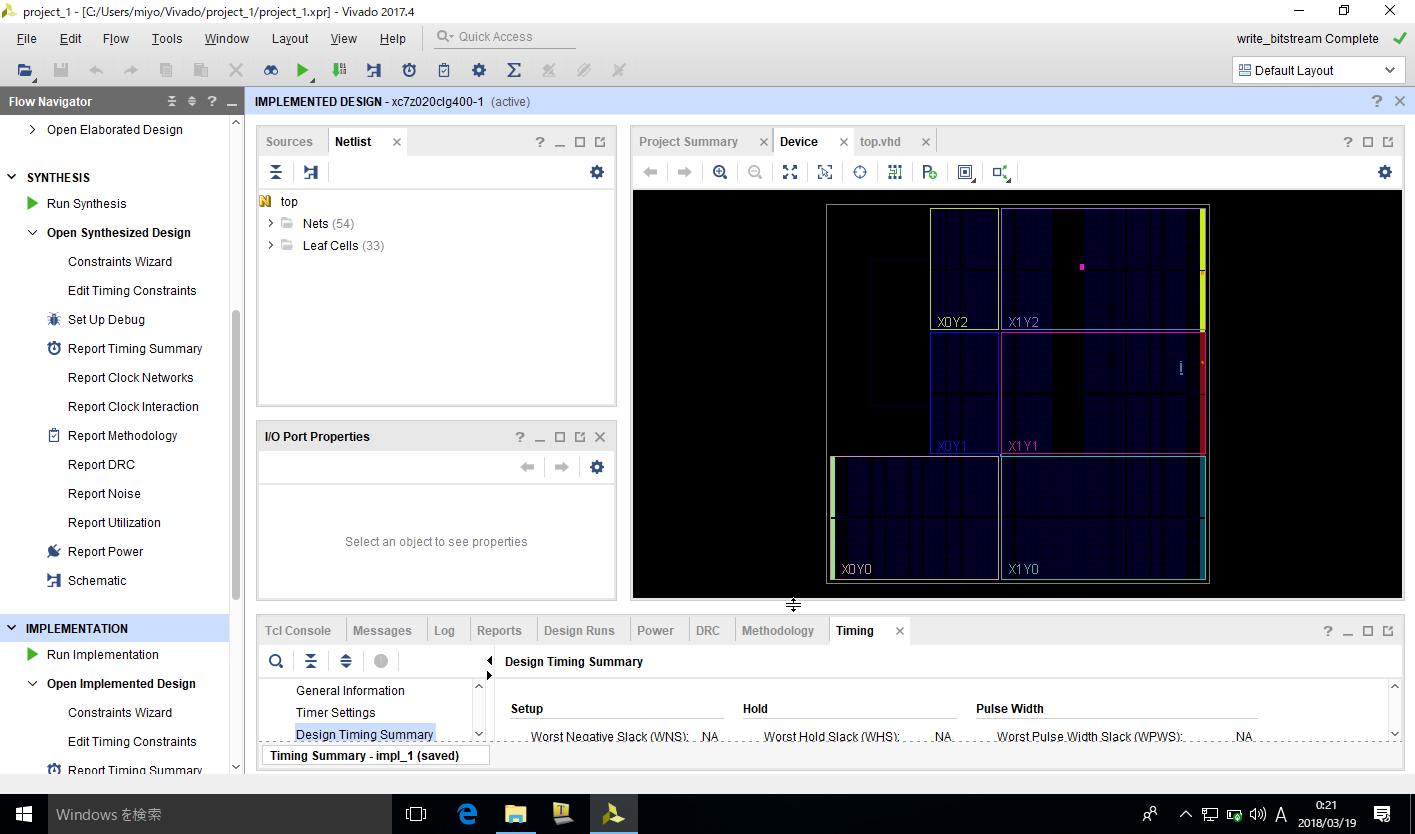
\includegraphics[width=.8\textwidth]{chapter03_figures/VirtualBox_Windows10_19_03_2018_00_21_16.png}
  \end{center}
  \caption{配置配線結果を開いてみたところ.右側の水色部分が使用しているハードウェアリソース}
 \end{figure}

 \begin{figure}[H]
  \begin{center}
   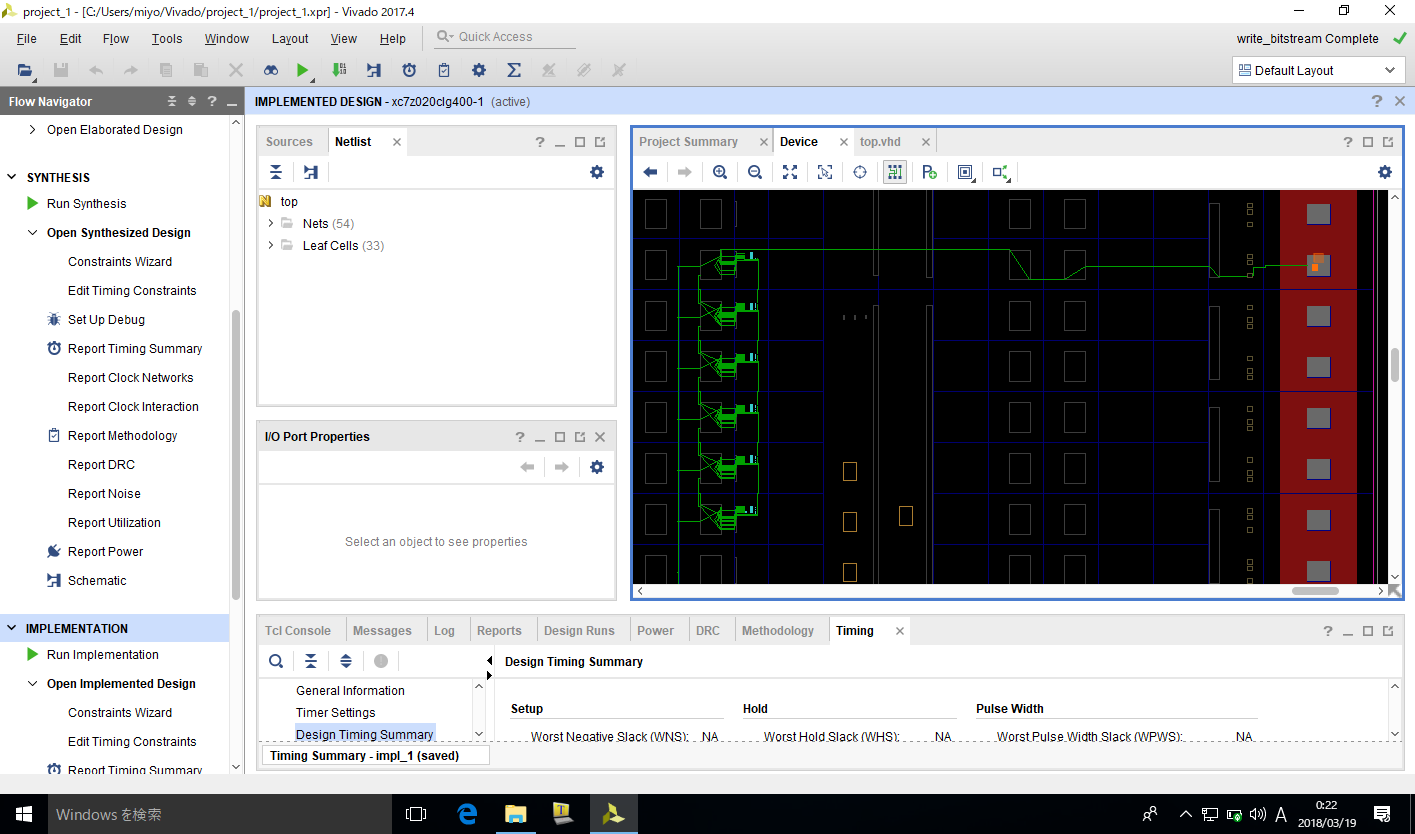
\includegraphics[width=.8\textwidth]{chapter03_figures/VirtualBox_Windows10_19_03_2018_00_22_24.png}
  \end{center}
  \caption{接続パスを表示し,拡大してみたところ}
 \end{figure}


\subsection{実機での動作確認}

できあがったデータをFPGAボードにダウンロードして動作させてみましょう.

まずは,FPGAとパソコンをUSBケーブルで接続します.ここで,JP5のジャンパをJTAGに,JP16のジャンパをUSB側にセットしておいてください.

 \begin{figure}[H]
  \begin{center}
   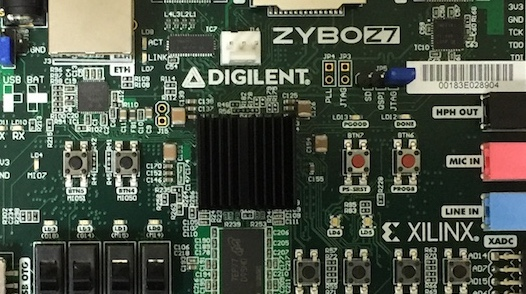
\includegraphics[width=.8\textwidth]{chapter03_figures/IMG_0002.JPG}
  \end{center}
  \caption{FPGAとパソコンをUSBケーブルで接続.JP5とJP16の位置にも注意}
 \end{figure}

書き込みの手順は次の通りです.

 \begin{figure}[H]
  \begin{center}
   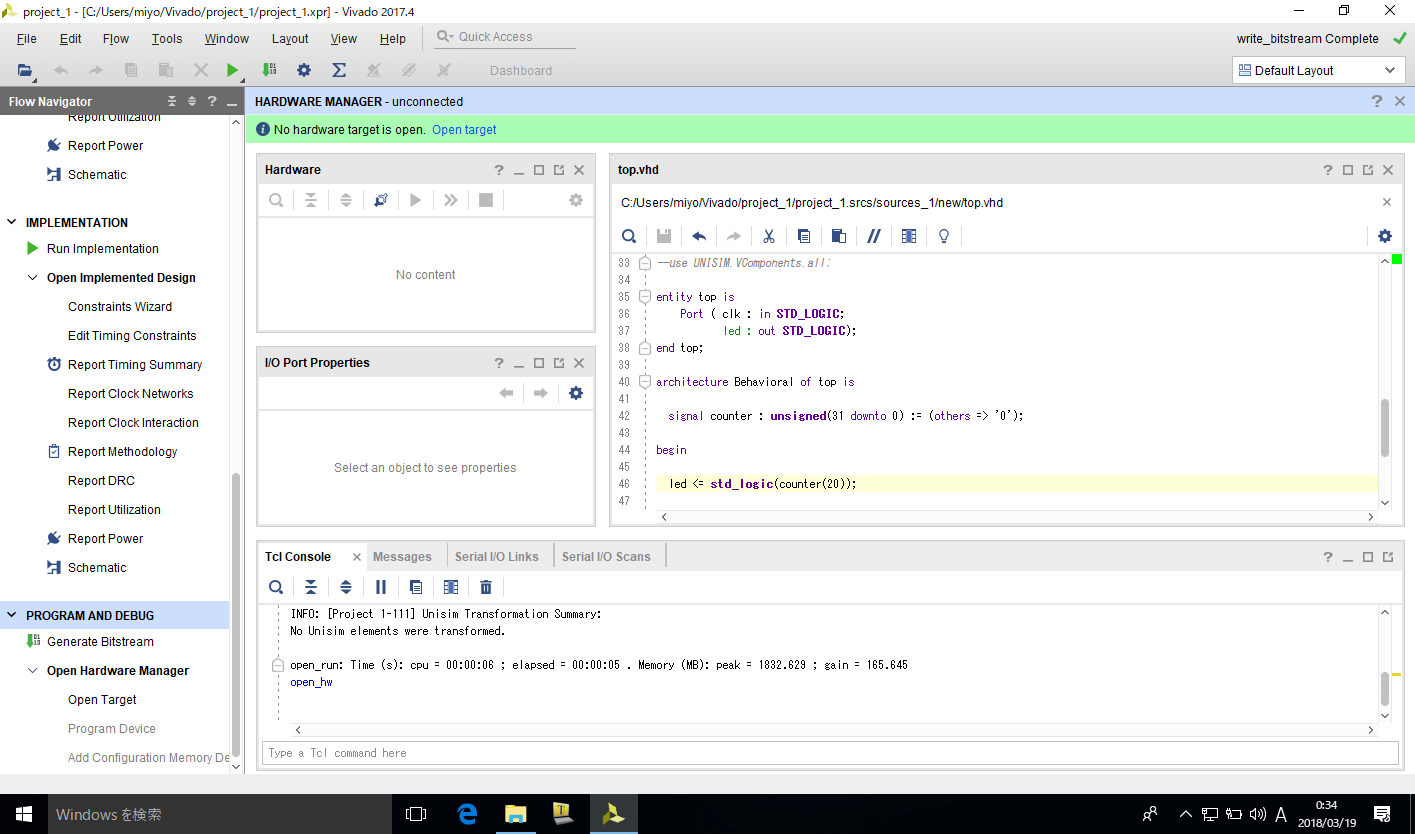
\includegraphics[width=.8\textwidth]{chapter03_figures/VirtualBox_Windows10_19_03_2018_00_34_35.png}
  \end{center}
  \caption{Navigator FlowでOpen Hardwareをクリックしたところ}
 \end{figure}

 \begin{figure}[H]
  \begin{center}
   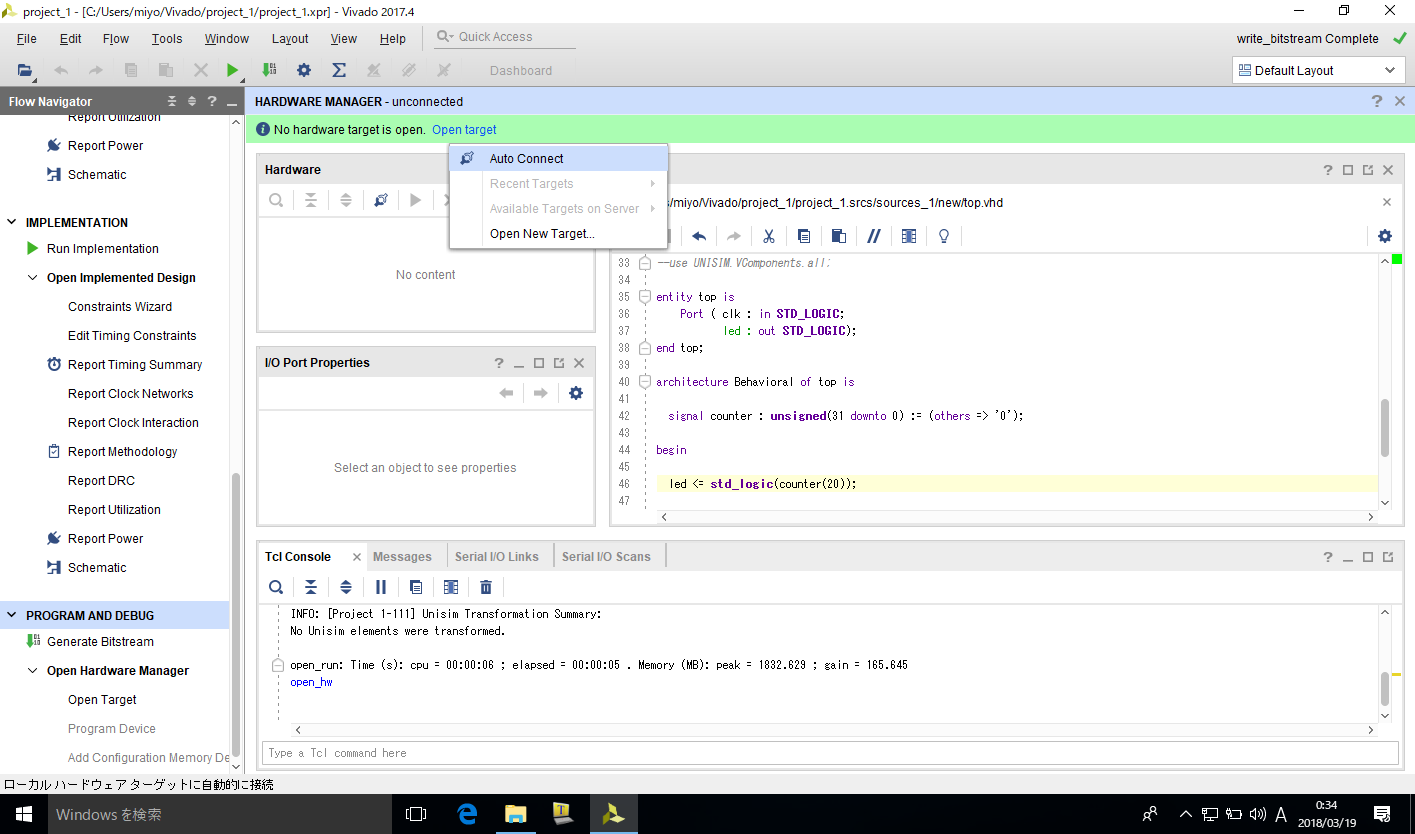
\includegraphics[width=.8\textwidth]{chapter03_figures/VirtualBox_Windows10_19_03_2018_00_34_45.png}
  \end{center}
  \caption{Open Targetをクリックし,Auto Connectをクリック}
 \end{figure}

 \begin{figure}[H]
  \begin{center}
   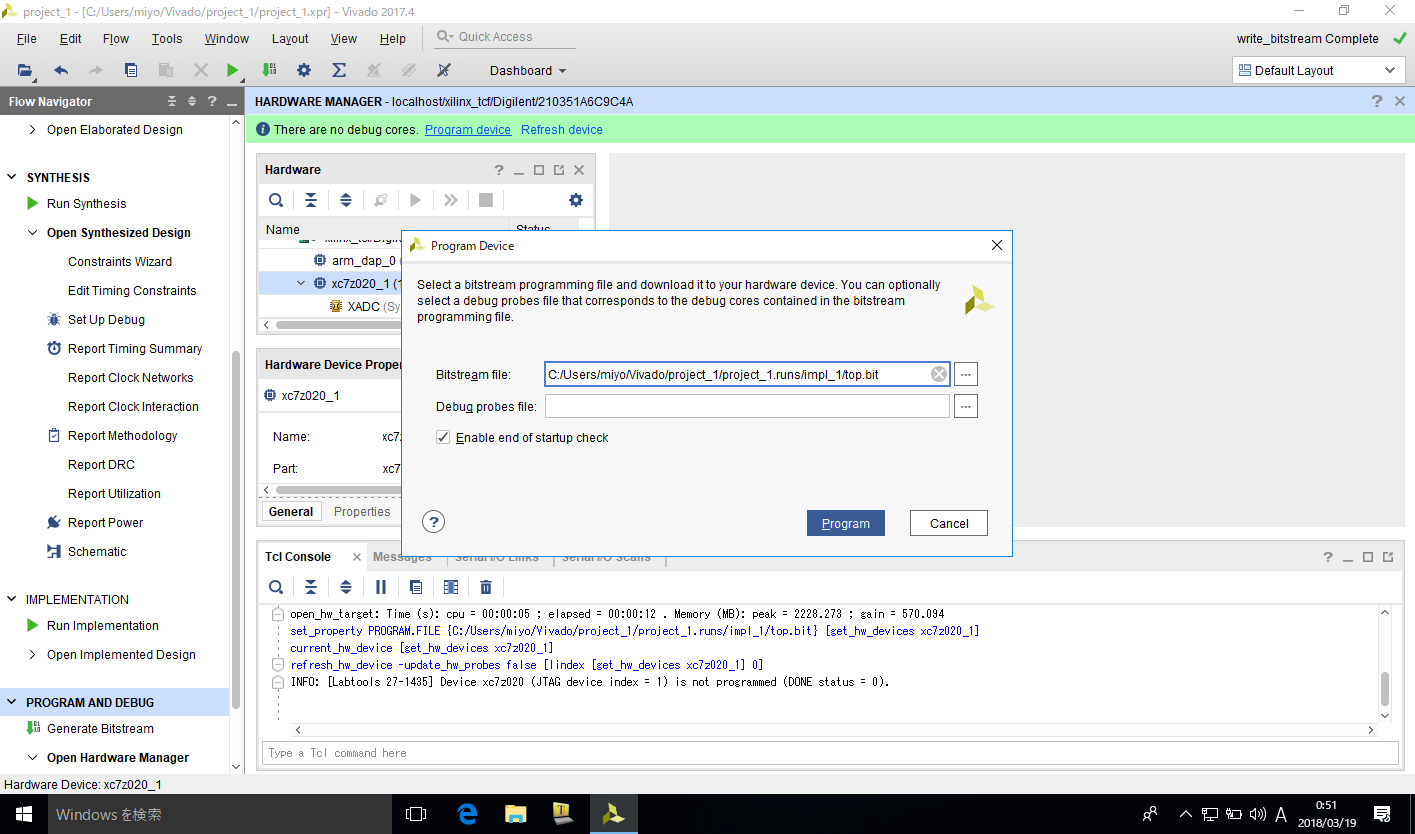
\includegraphics[width=.8\textwidth]{chapter03_figures/VirtualBox_Windows10_19_03_2018_00_51_49.png}
  \end{center}
  \caption{FPGAボードと接続できたら,Program Deviceをクリック.開いたファイルダイアログでOKをクリック.}
 \end{figure}

これでFPGAボード上のLED LD0が点滅するはずです.

\section{課題}
\begin{enumerate}
 \item 点滅の間隔を変えてみよう
 \item FPGA上のほかのLEDも点滅させてみよう
\end{enumerate}


\end{document}
